\subsection{典范双线性形式}

我们已经看到（第 1 号，命题 3），对称双线性形式

\[
(x, y) \mapsto \mathrm{B} _ {\mathrm{R}} (x, y) = \sum_ {\alpha \in \mathbb {R}} \langle \alpha^ {\prime}, x \rangle \langle \alpha^ {\prime}, y \rangle
\]

它在 V 上非退化且在 A(R) 下不变。交换 R 与 \(R^{\prime}\) 的作用，便得到，对称双线性形式 \((x^{*}, y^{*}) \mapsto \mathrm{B}_{\mathbb{R}^{\prime}}(x^{*}, y^{*}) = \sum_{\alpha \in \mathbb{R}^{\prime}} \langle \alpha, x^{*} \rangle \langle \alpha, y^{*} \rangle\) 在 \(V^{*}\) 上非退化且在 A(R) 下不变。

\(B_{R^{\prime}}\)（分别为 \(B_{R}\)）在 V（分别为 \(V^{*}\)）上的逆形式称为 V（分别为 \(V^{*}\)）上的典范双线性形式，记为 \(\Phi_{R}\)（分别为 \(\Phi_{R^{\prime}}\)）。它非退化且在 A(R) 下不变。令 \(\sigma\) 为从 V 到 \(V^{*}\) 且由 \(B_{R^{\prime}}\) 定义的同构。于是，对于 \(x \in V\) 和 \(y \in V\)：

\[
\Phi_ {R} (x, y) = B _ {R ^ {\prime}} (\sigma (x), \sigma (y)) = \sum_ {\alpha \in R} \langle \alpha , \sigma (x) \rangle \langle \alpha , \sigma (y) \rangle .
\]

但是 \(\langle \alpha, \sigma(x) \rangle = B_{R^{\prime}}(\sigma(\alpha), \sigma(x)) = \Phi_R(\alpha, x)\)。因此，

\[
\Phi_ {\mathsf {R}} (x, y) = \sum_ {\alpha \in \mathsf {R}} \Phi_ {\mathsf {R}} (\alpha , x) \Phi (\alpha , y).\tag{16}
\]

根据第 2 号命题 7，\(\Phi_{R}\) 是满足恒等式 (16) 且在 W(R) 下不变的唯一非零对称双线性形式。

对于 \(\beta \in \mathbb{R}\)，由 (16) 得

\[
\varPhi_ {\mathrm{R}} (\beta , \beta) = \sum_ {\alpha \in \mathrm{R}} \varPhi_ {\mathrm{R}} (\alpha , \beta) ^ {2} = \frac {1}{4} \varPhi_ {\mathrm{R}} (\beta , \beta) ^ {2} \sum_ {\alpha \in \mathrm{R}} n (\alpha , \beta) ^ {2},
\]

故

\[
4 \Phi_ {R} (\beta , \beta) ^ {- 1} = \sum_ {\alpha \in R} n (\alpha , \beta) ^ {2}.\tag{17}
\]

此外，根据第 1 号引理 2，对于 \(x, y \in V\)，有：

\[
\begin{array}{r l} & {\mathrm{B} _ {\mathrm{R}} (x, y) = \sum_ {\alpha \in \mathrm{R}} \varPhi_ {\mathrm{R}} \left(\frac {2 \alpha}{\varPhi_ {\mathrm{R}} (\alpha , \alpha)}, x\right) \left(\frac {2 \alpha}{\varPhi_ {\mathrm{R}} (\alpha , \alpha)}, y\right)} \\ & {\qquad = 4 \sum_ {\alpha \in \mathrm{R}} \varPhi_ {\mathrm{R}} (\alpha , x) \varPhi_ {\mathrm{R}} (\alpha , y) \varPhi_ {\mathrm{R}} (\alpha , \alpha) ^ {- 2}.} \end{array}
\]

由此，若 \(R\) 不可约，则存在常数 \(\gamma(R) > 0\)，使得

\[
\sum_ {\alpha \in R} \Phi_ {R} (\alpha , x) \Phi_ {R} (\alpha , y) \Phi_ {R} (\alpha , \alpha) ^ {- 2} = \gamma (R) \Phi_ {R} (x, y).\tag{18}
\]

根据 \(\gamma (\mathbb{R})\) 的定义，有 \(B_{\mathbb{R}}(x,y) = 4\gamma (\mathbb{R})\Phi_{\mathbb{R}}(x,y)\)，故

\[
\Phi_ {\mathrm{R} ^ {\prime}} \left(x ^ {*}, y ^ {*}\right) = (4 \gamma (\mathrm{R})) ^ {- 1} \mathrm{B} _ {\mathrm{R} ^ {\prime}} \left(x ^ {*}, y ^ {*}\right)
\]

对于 \(x^{*},y^{*}\in V^{*}\)。这证明了 \(\gamma (\mathsf{R}) = \gamma (\mathsf{R}^{\prime})\)。另一方面，对于 \(\beta \in \mathbb{R}\)，

\[
\begin{array}{c} \Phi_ {\mathrm{R} ^ {\prime}} (\beta^ {\prime}, \beta^ {\prime}) = (4 \gamma (\mathrm{R})) ^ {- 1} \sum_ {\alpha \in \mathfrak {R}} \langle \beta^ {\prime}, \alpha \rangle^ {2} \\ = \gamma (\mathrm{R}) ^ {- 1} \sum_ {\alpha \in \mathbb {R}} \frac {\Phi_ {\mathrm{R}} (\alpha , \beta) ^ {2}}{\Phi_ {\mathrm{R}} (\beta , \beta) ^ {2}} \end{array}
\]

所以，根据 (16)，

\[
\Phi_ {\mathrm{R} ^ {\prime}} (\beta^ {\prime}, \beta^ {\prime}) = \gamma (\mathrm{R}) ^ {- 1} \Phi_ {\mathrm{R}} (\beta , \beta) ^ {- 2} \Phi_ {\mathrm{R}} (\beta , \beta)
\]

或最后

\[
\Phi_ {R} (\beta , \beta) \Phi_ {R ^ {\prime}} (\beta^ {\prime}, \beta^ {\prime}) = \gamma (R) ^ {- 1}.\tag{19}
\]

此外，若 \(\mathbb{R}\) 的所有根相对于 \(\lambda\) 都具有相同长度（长度由 \(\varPhi_{\mathbb{R}}\) 给出），则 (16) 和 (18) 表明

\[
\gamma (R) = \lambda^ {- 4}.\tag{20}
\]

此外，若 \(h\) 是 \(W\) 的 Coxeter 数，则第五章第 6 节第 2 号定理 1 的推论表明：

\[
h \Phi_ {R} (x, x) = \sum_ {\alpha \in R} \left(x, \frac {\alpha}{\lambda}\right) ^ {2} \text {   for   all   } x \in V.
\]

与 (16) 比较，得到

\[
\lambda = h ^ {- 1 / 2} \text { or } \gamma (\mathrm{R}) = h ^ {2}.\tag{21}
\]

最后，公式 (19) 表明，\(R^{\prime}\) 的根具有长度 \(\lambda\)（相对于 \(\Phi_{R^{\prime}}\)）。

\section{仿射韦伊群}

在本段中（第 5 号除外），记 R 为实向量空间 V 中的约化根系。记 W 为 R 的韦伊群；将其视为 V 的对偶 \(V^{*}\) 的自同构群（\(\S\) 1 节，第 1 号），并在 \(V^{*}\) 上取一个 W 不变的标量积。令 E 为以 \(V^{*}\) 为底空间的仿射空间；对于 \(v \in V^{*}\)，记 \(t(v)\) 为 E 沿向量 v 的平移。最后，记 P（分别为 Q）为平移 \(t(v)\) 所成的群，其中向量 v 属于权群 \(\mathrm{P}(\mathrm{R}^{\prime})\)（分别为根权群 \(\mathrm{Q}(\mathrm{R}^{\prime})\)），且这些权群属于 R 的对偶根系 \(R^{\prime}\)。

\subsection{仿射韦伊群}

对于 \(\alpha \in \mathbb{R}\) 和 \(k\in \mathbf{Z}\)，令 \(\mathrm{L}_{\alpha ,k}\) 为 E 中由下式定义的超平面：

\[
\mathrm{L} _ {\alpha , k} = \{x \in \mathrm{E} | \langle \alpha , x \rangle = k \}
\]

并令 \(s_{\alpha, k}\) 为关于 \(L_{\alpha, k}\) 的正交反射。于是

\[
s _ {\alpha , k} (x) = x - (\langle \alpha , x \rangle - k) \alpha^ {\prime} = s _ {\alpha , 0} (x) + k \alpha^ {\prime}
\]

对所有 \(x \in E\) 成立。换言之，

\[
s _ {\alpha , k} = t (k \alpha^ {\prime}) \circ s _ {\alpha}\tag{1}
\]

其中 \(s_{\alpha}\) 是关于超平面 \(L_{\alpha} = L_{\alpha,0}\) 的正交反射，即与根 \(\alpha\) 相关联的反射。

公式 (1) 表明，\(s_{\alpha, k}\) 不依赖于所选的标量积。

定义 1. 称由反射 \(s_{\alpha,k}\)（其中 \(\alpha \in R\) 且 \(k \in Z\)）生成的 E 的仿射变换群为根系 R 的仿射韦伊群，记为 \(\mathrm{W}_{a}(\mathrm{R})\)（或简记为 \(W_{a}\)）。

命题 1. 群 \(\mathrm{W}_a\) 是 \(\mathrm{W}\) 与 \(\mathrm{Q}\) 的半直积。

由于 W 由反射 \(s_{\alpha}\) 生成，所以 W 包含于 \(W_{a}\) 中。另一方面，\(t(\alpha^{\prime}) = s_{\alpha,1} \circ s_{\alpha}\)（当 \(\alpha \in R\) 时），这说明 \(Q \subseteq W_{a}\)。

由于 W 保持 \(Q(R^{\prime})\) 不变（\(\S\) 1，第 9 号），由 W 和 Q 生成的仿射变换群 G 是 W 与 Q 的半直积。由上可知 \(G \subseteq W_{a}\)，且根据 (1) 有 \(s_{\alpha,k} \in G\)（对所有 \(\alpha \in R\) 和 \(k \in Z\)）。因此 \(W_{a} = G\)。

命题 2. 群 \(W_{a}\) 赋予离散拓扑后在 E 上适当作用，并置换超平面 \(L_{\alpha,k}\)（其中 \(\alpha \in R\) 且 \(k \in Z\)）。

由于 \(Q(R^{\prime})\) 是 \(V^{*}\) 的离散子群，群 Q 在 E 上适当作用。因此 \(W_{a} = W.Q\) 也如此，因为 W 是有限群。此外，对于 \(\alpha, \beta \in R\) 和 \(k \in Z\)：

\[
s _ {\beta} (\mathrm{L} _ {\alpha , k}) = \mathrm{L} _ {\gamma , k} \text {with} \gamma = s _ {\beta} (\alpha) \in \mathrm{R},
\]

\[
t (\beta^ {\prime}) \left(\mathrm{L} _ {\alpha , k}\right) = \mathrm{L} _ {\alpha , k + n (\alpha , \beta)},
\]

其中 \(n(\alpha, \beta) = \langle \beta^{\prime}, \alpha \rangle\) 是整数，故得第二个断言。

因此可以将第五章第 3 节关于 \(W_{a}\) 在 E 上作用的结果应用于此。为避免与 W 在 \(V^{*}\) 中的室混淆，我们把由超平面系 \(L_{\alpha,k}\)（其中 \(\alpha \in R\) 且 \(k \in Z\)）在 E 中确定的室称为小室。于是 \(W_{a}\) 在小室集合上单纯传递地作用，而小室的闭包是 \(W_{a}\) 在 E 上作用的基本域（第五章第 3 节第 2 号定理 1 及第 3 号定理 2）。显然，W 群可与 \(U(W_{a})\)（\(W_{a}\) 在 \(V^{*}\) 的正交群中的典范像）相识别（参见第五章第 3 节第 6 号）。由此 \(W_{a}\) 是本质的（第五章第 3 节第 7 号），且 \(W_{a}\) 不可约当且仅当根系 R 不可约（第 1 节第 2 号命题 5 的推论）。若 R 不可约，每个小室都是开单纯形（第五章第 3 节第 9 号命题 8）。一般情况下，仿射空间 E 的典范乘积分解（第五章第 3 节第 8 号）对应于 R 分解为不可约分支。特别地，小室是开单纯形的乘积。

还要注意，第五章第 3 节第 2 号定理 1 的推论表明，\(s_{\alpha,k}\) 是 \(\mathbf{W}_a\) 中唯一的反射。

\subsection{权与特殊权}

命题 3. \(W_{a}\) 的特殊点（第五章第 3 节第 10 号定义 1）正是 \(R^{\prime}\) 的权。

设 \(x_0 \in E\) 且 \(\alpha \in R\)。平行于 Ker \(\alpha\) 且经过 \(x_0\) 的超平面 L 的方程为 \(\langle \alpha, x \rangle = \langle \alpha, x_0 \rangle\)。要使它等于某个 \(L_{\beta,k}\)，一方面必须 \(\alpha\) 与 \(\beta\) 成比例，因 R 是约化的，故 \(\beta = \pm \alpha\)；另一方面必须 \(\langle \alpha, x_0 \rangle\) 为整数。立即得到，\(x_0\) 是 \(W_a\) 的特殊点，当且仅当 \(\langle \alpha, x_0 \rangle \in Z\) 对所有 \(\alpha \in R\) 成立，换言之，当且仅当 \(x_0 \in P(R^{\prime})\)（第 1 节，第 9 号）。

推论。(i) 若 \(\overline{\omega} \in \mathrm{P}(\mathbb{R}^{\prime})\)，则存在一个小室 C，使得 \(\overline{\omega}\) 是 \(\overline{\mathbb{C}}\) 的一个极点。

\begin{enumerate}
\def\labelenumi{(\roman{enumi})}
\setcounter{enumi}{1}
\tightlist
\item
  若 \(\mathbf{C}\) 是一个小室，则 \(\overline{\mathbf{C}} \cap \mathbf{Q}(\mathbb{R}^{\prime})\) 退化为一个点，且该点是 \(\overline{\mathbf{C}}\) 的一个极点。
\end{enumerate}

这由命题 3、第五章第 3 节第 10 号命题 11 的推论以及第五章第 3 节第 10 号命题 12 可得。

命题 4. 设 \(C'\) 是 \(R'\) 的一个室。

\begin{enumerate}
\def\labelenumi{(\roman{enumi})}
\item
  存在唯一的小室 C 包含于 \(\mathbf{C}'\)，使得 \(0\in \overline{\mathbf{C}}\)
\item
  \(w(\overline{\mathbf{C}})\)（\(w\in \mathrm{W}\)）的并，是 E 中 0 的一个邻域。
\item
  \(\mathbf{C}'\) 的每一面壁都是 \(\mathbf{C}\) 的一面壁。
\end{enumerate}

这由第五章第 3 节第 10 号命题 11 可得。

现在假设 \(R\) 不可约。设 \((\alpha_i)_{i\in I}\) 是 \(R\) 的一组基（第 1 节，第 5 号，定义 2），并设 \((\overline{\omega}_i)_{i\in I}\) 是对偶基。\(\overline{\omega}_i\) 是 \(R^{\prime}\) 的基本权，属于室 \(D'\)；此室是 \(R^{\prime}\) 中对应于基 \((\alpha_i)\) 的室。令

\[
\tilde {\alpha} = \sum_ {i \in \mathrm{I}} n _ {i} \alpha_ {i}
\]

为 \(\mathbf{R}\) 的最高根（第 1 节，第 8 号），并令 \(\mathbf{J}\) 为由 \(i \in \mathbf{I}\) 且满足 \(n_i = 1\) 的 i 所成的集合。

命题 5. 设 \(\mathbf{C}\) 是包含于 \(\mathbf{C}'\) 且其闭包包含 0 的小室（命题 4）。

\begin{enumerate}
\def\labelenumi{(\roman{enumi})}
\tightlist
\item
  C 是由 \(x \in E\) 组成的集合，其中 \(\langle\alpha_{i}, x\rangle > 0\)（对所有 \(i \in I\)），且有 \(\langle\tilde{\alpha}, x\rangle < 1\)。
\item
  集合 \(\overline{C} \cap P(R^{\prime})\) 由 0 以及 \(\overline{\omega}_{i}\)（\(i \in J\)）组成。
\end{enumerate}

令 D 为由 \(x \in E\) 组成且满足 \(\langle\tilde{\alpha}, x\rangle < 1\) 的集合，并置 \(C_{1} = C' \cap D\)。由于 \(0 \in \overline{C}\)，有 \(C \subseteq D\)，从而 \(C \subseteq C_{1}\)。我们将证明，对于所有 \(\alpha \in R\) 和 \(k \in Z\)，集合 C 与 \(C_{1}\) 位于超平面 \(L_{\alpha,k}\) 的同一侧。这将证明 \(C_{1} \subseteq C\)，从而建立断言 (i)。若 k = 0，则整个室 \(C'\) 位于 \(L_{\alpha,0}\) 的一侧，在此情形断言成立。若 \(k \neq 0\)，将 \(\alpha\) 替换为 \(-\alpha\) 后可设 k \textgreater{} 0。于是，在 C 上有 \(\langle\alpha, x\rangle < k\)，这是因为 \(0 \in \overline{C}\)。另一方面，\(\tilde{\alpha} - \alpha\) 在 \(C'\) 上为正（第 1 节，第 8 号，命题 25）。因此，对 \(y \in C_{1}\)，有 \(\langle\alpha, y\rangle \leqslant \langle\tilde{\alpha}, y\rangle < 1 \leqslant k\)。所以 C 与 \(C_{1}\) 位于 \(L_{\alpha,k}\) 的同一侧。

现在设 \(\overline{\omega} \in P(R^{\prime})\)。则 \(\overline{\omega} = \sum_{i} p_i \overline{\omega}_i\)，其中 \(p_i \in \mathbf{Z}\)（第 1 节，第 10 号），并且 \(\overline{\omega} \in \overline{C'}\) 当且仅当整数 \(p_i\) 为正。若 \(\overline{\omega} \in \overline{C'}\)，则 \(\overline{\omega} \in \overline{C}\) 当且仅当 \(\langle \tilde{\alpha}, \overline{\omega} \rangle = \sum_{i} n_i p_i\) 满足 \(\leqslant 1\)，故得 (ii)。

推论。小室 C 是一个开单纯形，其顶点为 0 以及 \(\overline{\omega}_i / n_i\)（\(i \in I\)）。

这由 (i) 得出。

\subsection{\texorpdfstring{\(W_{a}\) 的正规化子}{W\_a 的正规化子}}

本号中，我们假设 V 上所选的标量积不仅在 W 下不变，而且在整个群 A(R) 下不变。我们认同 A(R) 与 A(R \(^{\prime}\)）。

令 G 为 \(W_{a}\) 在仿射欧几里得空间 E 的位移群中的正规化子。若 g 是 E 的一个位移，s 是关于超平面 L 的正交反射，则位移 \(gsg^{-1}\) 是关于超平面 \(g(L)\) 的正交反射。因此，G 正是置换超平面 \(L_{\alpha,k}\)（其中 \(\alpha \in R\) 且 \(k \in Z\)）的 E 的位移所成的集合。

现在，E 的自同构群是 \(V^{*}\) 的正交群 U 与平移群 T 的半直积。若 \(u \in U\) 且 \(v \in V^{*}\)，则超平面 \(L_{\alpha,k}\) 在 \(g = u \circ t(v)\) 下变为方程为

\[
\langle^ {t} u ^ {- 1} (\alpha), x \rangle = k + \langle \alpha , v \rangle .
\]

因此，\(g \in \mathbf{G}\) 当且仅当，一方面 \({}^t u\) 置换这些根，亦即属于 \(\mathrm{A(R)}\)；另一方面有 \(\langle \alpha, v \rangle \in \mathbf{Z}\)（对所有 \(\alpha \in \mathbb{R}\)），即 \(v \in \mathrm{P(R^{\prime})}\)。换言之，群 \(G\) 是 \(A(R)\) 与 \(P\) 的半直积。由于 \(Q \subseteq P\) 且 \(W \subseteq A(R)\)，商群 \(G / W_a\) 是 \(A(R)/W\) 与 \(P(R^{\prime})/Q(R^{\prime})\) 的半直积；容易验证，\(A(R)/W\) 在 \(P(R^{\prime})/Q(R^{\prime})\) 上的相应作用就是典范作用（第 1 节，第 9 号）。

记 \(W_{a}^{\prime}\) 为由 W 与 P 的半直积构成的 G 的子群。这是 G 的正规子群，且 \(G/W_{a}^{\prime}\) 典范同构于 \(A(R)/W\)；此外，从 \(P(R^{\prime})\) 到 \(W_{a}^{\prime}/W_{a}\) 的典范映射通过取商给出 \(P(R^{\prime})/Q(R^{\prime})\) 到 \(W_{a}^{\prime}/W_{a}\) 的一个同构。

现在令 C 为 E 的一个小室，令 \(G_{C}\) 为由元素 \(g \in G\)（满足 \(g(\mathrm{C}) = \mathrm{C}\)）所成的子群。由于 \(W_{a}\) 在小室上单纯传递地作用，群 G 是 \(G_{C}\) 与 \(W_{a}\) 的半直积。相应的从 \(G/W_{a}\) 到 \(G_{C}\) 的同构尤其给出从 \(\mathrm{P}(\mathrm{R}^{\prime})/\mathrm{Q}(\mathrm{R}^{\prime})\) 到群 \(\Gamma_{C} = G_{C} \cap W_{a}^{\prime}\) 的一个典范同构。

假设 R 不可约，并保留第 2 号命题 5 的记号。置 \(R_{0} = R\)，并令 \(R_{i} (i \in I)\) 为由 \(a_{j}\)（\(j \neq i\)）生成的根系。对于 i = 0（分别对于 \(i \in I\)），令 \(w_{i}\) 为 \(W(R_{i})\) 中的唯一元素（将其视为 W 的子群），它把 \(R_{i}\) 相对于基 \((\alpha_{j})_{j \neq i}\) 的正根变为负根（第 1 节，第 6 号，命题 17 的推论 3）。

命题 6. 对所有 \(i \in \mathbf{J}\)，元素 \(\gamma_i = t(\overline{\omega}_i)w_i w_0\) 属于 \(\Gamma_{C}\)，且映射 \(i \mapsto \gamma_i\) 是从 \(\mathbf{J}\) 到 \(\Gamma_{C} - \{1\}\) 的双射。

首先注意，根 \(w_{i}(\tilde{\alpha})\) 具有形式

\[
n _ {i} \alpha_ {i} + \sum_ {j \neq i} b _ {i j} \alpha_ {j},
\]

因而是正根。

我们证明，若 \(i \in \mathrm{J}\)，则 \(\gamma_i \in \Gamma_{C}\)。事实上，设 \(a \in \mathrm{C}\) 且 \(b = \gamma_i(a)\)。对于 \(1 \leqslant j \leqslant l\) 且 \(j \neq i\)，

\[
\begin{array}{r l} \langle b, \alpha_ {j} \rangle & = \langle \overline {{\omega}} _ {i} + w _ {i} w _ {0} (a), \alpha_ {j} \rangle \\ & = \langle w _ {0} (a), w _ {i} (\alpha_ {j}) \rangle > 0 \end{array}\tag{2}
\]

因为 \(w_0(a) \in -\mathbf{C}'\)，且 \(w_i(\alpha_j)\) 为负根。另一方面，

\[
\langle b, \alpha_ {i} \rangle = 1 + \left\langle w _ {0} (a), w _ {i} (\alpha_ {i}) \right\rangle \geqslant 1 + \left\langle w _ {0} (a), \tilde {\alpha} \right\rangle > 0\tag{3}
\]

因为 \(w_0(a) \in -\mathbf{C}'\)，\(\tilde{\alpha} - w_i(\alpha_i)\) 在 \(-\mathbf{C}'\) 上取负值，且 \(\langle w_0(a), \tilde{\alpha} \rangle > -1\)。最后，

\[
\langle b, \tilde {\alpha} \rangle = n _ {i} + \left\langle w _ {0} (a), w _ {i} (\tilde {\alpha}) \right\rangle = 1 + \left\langle w _ {0} (a), w _ {i} (\tilde {\alpha}) \right\rangle <   1\tag{4}
\]

因为 \(w_0(a) \in -\mathbf{C}'\)，且 \(w_i(\tilde{\alpha})\) 是正根。于是关系 (2)、(3) 和 (4) 蕴含 \(b \in \mathbf{C}\)，从而 \(\gamma_i \in \Gamma_{C}\)。显然，映射 \(i \mapsto \gamma_i\) 是单射，因为 \(\gamma_i(0) = \overline{\omega}_i\)。最后，设 \(\gamma \in \Gamma_{C}\) 且 \(\gamma \neq 1\)，并令 \(\gamma = tw\)，其中 \(t \in \mathbf{P}\) 且 \(w \in W\)。于是 \(t \neq 1\)，因为 \(\Gamma_{C} \cap W = \{1\}\)。另一方面，\(t(0) = \gamma(0) \in \overline{\mathbf{C}} \cap P(\mathbf{R}^{\prime})\)，命题 5 蕴含存在 \(i \in J\) 使得 \(t(0) = \overline{\omega}_i\)。于是 \(\gamma_i^{-1}\gamma(0) = 0\)，故 \(\gamma = \gamma_i\)，因为 \(\Gamma_{C} \cap W = \{1\}\)。证明完毕。

推论。 \((\bar{\omega}_i)_{i\in J}\) 在 \(\mathrm{P}(\mathbb{R}^{\prime})\) 中构成 \(\mathrm{P}(\mathbb{R}^{\prime}) / \mathrm{Q}(\mathbb{R}^{\prime})\) 的非零元素的一组代表元。

事实上，若将 \(\Gamma_{C}\) 与 \(\mathrm{P}(\mathbb{R}^{\prime}) / \mathrm{Q}(\mathbb{R}^{\prime})\) 认同，则元素 \(\gamma_{i}\) 对应于 \(\overline{\omega}_{i}\) 模 \(\mathrm{Q}(\mathbb{R}^{\prime})\) 的陪集。

备注。1）映射 \(\gamma \mapsto \gamma(0)\) 是从 \(\Gamma_{C}\) 到 \(\overline{\mathrm{C}} \cap \mathrm{P}(\mathrm{R}^{\prime})\) 的双射。

\begin{enumerate}
\def\labelenumi{\arabic{enumi})}
\setcounter{enumi}{1}
\tightlist
\item
  若 E 只赋予其仿射结构，则群 G 也是 \(W_{a}\) 在 E 的自同构群中的正规化子（参见习题 3）。
\end{enumerate}

\subsection{应用：韦伊群的阶}

引理 1. 设 X 是一个在无穷远处可数的局部紧空间，G 是连续且适当地作用在 X 上的群，\(\mu\) 是 X 上的 G 不变测度，G' 是 G 的子群，U 和 U' 是 X 中测度有限且非零的两个开子集。假设对于 \(s \in G\) 的 sU（分别为 \(s'U'\)，其中 \(s' \in G'\)）两两不交，且它们的并集的补集为零测集。则 G' 在 G 中的指数有限，并且 \((\mathrm{G} : \mathrm{G}') = \mu(\mathrm{U}') / \mu(\mathrm{U})\)。

设 \((s_{\lambda})_{\lambda \in \Lambda}\) 是 G 中 \(G'\) 的右陪集的一组代表元。令 \(U_1\) 为各 \(s_{\lambda}U\) 的并。于是，各 \(s'U_1\)（其中 \(s' \in G'\)）两两不交，且其并为 \(M = \bigcup_{s \in G} sU\)。令 \(M' = \bigcup_{s' \in G'} s'U'\)。\(U'\)（分别为 \(U_1\)）与 \(X - M'\)（分别为 \(X - M\)）的某个适当子集之并是显然 \(\mu\)-可测的 \(G'\) 的一个基本域。根据《积分》第七章第 2 节第 10 号定理 4 的推论，有 \(\mu(U') = \mu(U_1)\)。这证明了 \(\text{Card } \Lambda = (G : G')\) 有限，并且 \(\mu(U') = (\text{Card } \Lambda)\mu(U)\)。

命题 7. 假设 R 不可约。设 \(B = \{\alpha_{1}, \ldots, \alpha_{l}\}\) 是 R 的一组基，f 是 R 的连接指标（第 1 节，第 9 号），且 \(\tilde{\alpha} = n_{1}\alpha_{1} + \cdots + n_{l}\alpha_{l}\) 是 R 的最高根（相对于 B 所定义的序）。则 W 的阶等于

\[
(l!) n _ {1} n _ {2} \dots n _ {l} f.
\]

设 \((\overline{\omega}_{1},\ldots,\overline{\omega}_{l})\) 是与 B 对偶的 P(R \(^{\prime}\) ) 的一组基。根据命题 5 的推论，以 \(0,n_{1}^{-1}\overline{\omega}_{1},\ldots,n_{l}^{-1}\overline{\omega}_{l}\) 为顶点的开单纯形 C 是 E 的一个小室。在加法群 V* 上取 Haar 测度 \(\mu\)。令 A 为由形如 \(\xi_{1}\overline{\omega}_{1}+\cdots+\xi_{l}\overline{\omega}_{l}\) 的 V* 中元素组成的集合，其中 \(0<\xi_{i}<1\)（当 \(i=1,\ldots,l\) 时）。根据《积分》第七章第 1 节第 10 号命题 15 的推论 2，

\[
\mu (\mathrm{A}) / \mu (\mathrm{C}) = (l!) n _ {1} n _ {2} \dots n _ {l}.\tag{5}
\]

另一方面，令 \(A'\) 为 \(V^{*}\) 中形如

\[
\xi_ {1} \alpha_ {1} ^ {\prime} + \dots + \xi_ {l} \alpha_ {l} ^ {\prime},
\]

其中 \(0 < \xi_i < 1\) 对 \(i = 1, \ldots, l\)。由于 \((\alpha_1', \ldots, \alpha_l')\) 是 \(\mathbf{Z}\)-模 \(\mathrm{Q}(\mathrm{R}^{\prime})\) 的一组基，可以在 \(\mathrm{X} = \mathrm{V}^*\)、\(\mathrm{G} = \mathrm{W}_a\)、\(\mathrm{G}' = \mathrm{Q}\)、\(\mathrm{U} = \mathrm{C}\) 和 \(\mathrm{U}' = \mathrm{A}'\) 的情况下应用引理 1。这给出

\[
\mu \left(\mathrm{A} ^ {\prime}\right) / \mu (\mathrm{C}) = \left(\mathrm{W} _ {a}: \mathrm{Q}\right) = \text { Card   W }.\tag{6}
\]

最后，再次应用引理 1，取 \(\mathrm{X} = \mathrm{V}^*\)、\(\mathrm{G} = \mathrm{P}\)、\(\mathrm{G}' = \mathrm{Q}\)、\(\mathrm{U} = \mathrm{A}\) 和 \(\mathrm{U}' = \mathrm{A}'\)。这给出

\[
\mu (A ^ {\prime}) / \mu (A) = (P: Q) = (P (R ^ {\prime}): Q (R ^ {\prime})) = f.\tag{7}
\]

比较公式 (5)、(6) 和 (7)，命题即得。

\subsection{根系与由反射生成的群}

命题 8. 设 F 是一个 l 维实 Hilbert 空间。令 H 为 F 的仿射超平面集，G 为由正交反射 \(s_{H}\)（关于超平面 \(H \in H\)）生成的群。假设第五章第 3 节的条件成立（即都有 \(g(H) \in H\)（对所有 \(H \in H\) 和 \(g \in G\)），且 G 在 F 上适当作用）。还假设 0 是 G 的一个特殊点，且属于 G 的平移群 T 的秩为 l。则在 \(V = F^{*}\) 中存在唯一的约化根系 R，使得从 F 到 \(V^{*}\) 的典范同构将 G 变为 R 的仿射韦伊群 \(W_{a}\)。

首先注意，关于 T 的假设蕴含 G 是本质的：否则仿射空间 F 将分解为乘积 \(F_{0} \times F_{1}\)，其中 \(\dim F_{1} < l\)，而群 G 可与在 \(F_{1}\) 上适当作用的一个位移群相识别（第五章第 3 节第 8 号命题 6），于是 T 的秩不会是 l。

令 \(\mathfrak{H}_0\) 为 \(\mathbf{H} \in \mathfrak{H}\) 中满足 \(0 \in \mathbf{H}\) 的元素所成的集合。对于 \(\mathbf{H} \in \mathfrak{H}_0\)，令 \(\mathfrak{H}_{\mathbf{H}}\) 为 \(\mathfrak{H}\) 中平行于 \(\mathbf{H}\) 的元素所成的集合。由于 0 是特殊点，\(\mathfrak{H}\) 是各 \(\mathfrak{H}_{\mathbf{H}}\)（其中 \(\mathbf{H} \in \mathfrak{H}_0\)）的并。由于 \(\mathbf{T}\) 的秩为 \(l\)，存在 \(v \in \mathbf{F}\)，使得沿向量 \(v\) 的平移属于 \(\mathbf{T}\) 且 \(v \notin \mathbf{H}\)。超平面 \(\mathbf{H} + kv\)（当 \(k \in \mathbf{Z}\) 时）两两不同且属于 \(\mathfrak{H}_{\mathbf{H}}\)。现在令 \(a\) 为 \(F\) 中与 \(\mathbf{H}\) 正交的单位向量；则 \(\mathbf{H} + (v|a)a \in \mathfrak{H}_{\mathbf{H}}\)，并且由于 \(\mathfrak{H}\) 是局部有限的（第五章第 1 节第 1 号引理 1），存在最小的实数 \(\lambda > 0\)，使得 \(\mathbf{H} + \lambda a \in \mathfrak{H}\)。我们将证明，\(\mathfrak{H}_{\mathbf{H}}\) 正是超平面 \(\mathbf{H} + k\lambda a\)（当 \(k \in \mathbf{Z}\) 时）所成的集合。事实上，

\[
\mathrm{H} ^ {\prime} = \mathrm{H} + \lambda a \in \mathfrak {H} _ {\mathrm{H}}
\]

而元素 \(s_{\mathrm{H}'} \circ s_{\mathrm{H}}\) 属于 \(\mathbf{G}\)，是沿向量 \(2\lambda a\) 的平移（第五章第 2 节第 4 号命题 5）。因此，\(\mathrm{H} + 2n\lambda a = (s_{\mathrm{H}'}s_{\mathrm{H}})^n(\mathrm{H})\) 和 \(\mathrm{H} + (2n + 1)\lambda a = (s_{\mathrm{H}'}s_{\mathrm{H}})^n(\mathrm{H}')\) 属于 \(\mathfrak{H}_{\mathrm{H}}\)。另一方面，若 \(\mathrm{L} \in \mathfrak{H}_{\mathrm{H}}\)，则存在 \(\xi \in \mathbf{R}\) 使得 \(\mathrm{L} = \mathrm{H} + \xi \lambda a\)，并且存在整数 \(n\) 使得

\[
\text { either } 2 n <   \xi \leqslant 2 n + 1, \text { or } 2 n - 1 <   \xi \leqslant 2 n.
\]

在第一种情形，\((s_{\mathrm{H}}s_{\mathrm{H}^{\prime}})^{n}(\mathrm{L}) = \mathrm{H} + (\xi -2n)\lambda a\)，其中

\[
0 <   (\xi - 2 n) \lambda \leqslant \lambda
\]

且由 \(\lambda\) 的定义可知 \(\xi = 2n + 1\)；在第二种情形，

\[
s _ {\mathrm{H}} (s _ {\mathrm{H}} s _ {\mathrm {H^ {\prime}}}) ^ {n} (\mathrm{L}) = \mathrm{H} + (2 n - \xi) \lambda a \text {with} 0 \leqslant (2 n - \xi) \lambda <   \lambda
\]

且由 \(\lambda\) 的定义可知 \(\xi = 2n\)。

由此，若 \(\alpha_{\mathrm{H}}\) 是 \(F\) 上满足下式的线性形式，

\[
\mathrm{H} ^ {\prime} = \left\{x \in \mathrm{F} \mid \langle \alpha_ {\mathrm{H}}, x \rangle = 1 \right\},
\]

\(\mathfrak{H}_{\mathrm{H}}\) 就是超平面 \(\mathrm{L}_{\alpha_{\mathrm{H}},k} = \{x\in \mathrm{F}\mid \langle \alpha_{\mathrm{H}},x\rangle = k\}\)（其中 \(k\in \mathbf{Z}\)）所成的集合，而 \(\alpha_{\mathrm{H}}\) 与 \(-\alpha_{\mathrm{H}}\) 是具有此性质的仅有的线性形式。

因此，只要证明由形如 \(\pm\alpha_{H}\) 的 V 中元素组成的集合 R 是 V 中的约化根系，命题即得证。

\begin{enumerate}
\def\labelenumi{\alph{enumi})}
\item
  我们证明条件 \((\mathrm{RS}_{\mathrm{I}})\)：显然 R 是有限集（因为 \(H_{0}\) 是有限集）且不含 0。此外，R 生成 V。事实上，若 \(x \in F\) 与 R 正交，则 \(x \in H\)（对所有 \(H \in H_{0}\)），且沿向量 x 的平移与 G 的每个元素交换。由于 G 是本质的，这蕴含 x = 0。
\item
  我们证明 \((\mathrm{RS}_{\mathrm{II}})\)。对于 \(v \in V\) 和 \(r \in R\)，如上置 \(L_{v,r} = \{x \in F | \langle v, x \rangle = r\}\)；若 \(\alpha \in R\)，置 \(H_{\alpha} = L_{\alpha,0}\)，并令 \(s_{\alpha}\) 为 \(s_{H_{\alpha}}\) 的转置。存在唯一的 \(\alpha' \in F\) 与 \(H_{\alpha}\) 正交且满足 \(\langle \alpha', \alpha \rangle = 2\)。于是 \(s_{H_{\alpha}} = s_{\alpha', \alpha}\) 且 \(s_{\alpha} = s_{\alpha, \alpha'}\)。对于 \(\beta \in R\)，
\end{enumerate}

\[
\mathrm{L} _ {s _ {\alpha} (\beta), 1} = s _ {\mathrm{H} _ {\alpha}} \left(\mathrm{L} _ {\beta , 1}\right) \in \mathfrak {H}
\]

且存在 \(\gamma \in \mathbb{R}\) 和 \(n\in \mathbf{N}^*\)，使得 \(\mathrm{L}_{s_{\alpha}(\beta),1} = \mathrm{L}_{\gamma ,n}\)。于是

\[
s _ {\mathrm{H} _ {\alpha}} (\mathrm{L} _ {\gamma , 1}) = \mathrm{L} _ {\beta , 1 / n}
\]

所以 \(1 / n\in \mathbf{Z}\)。于是 \(n = 1\) 且 \(s_{\alpha}(\beta) = \gamma \in \mathbb{R}\)。这证明了 \((\mathrm{RS}_{\mathrm{II}})\)。

\begin{enumerate}
\def\labelenumi{\alph{enumi})}
\setcounter{enumi}{2}
\tightlist
\item
  我们证明 \((\mathrm{RS}_{\mathrm{III}})\)。令 \(\alpha \in R\)，并置 \(H'_{\alpha} = L_{\alpha,1}\)。于是
\end{enumerate}

\[
\mathrm{H} _ {\alpha} ^ {\prime} = \mathrm{H} _ {\alpha} + (1 / 2) \alpha^ {\prime};
\]

由于平移 \(t(\alpha^{\prime})\)（沿向量 \(\alpha^{\prime}\)）是乘积 \(s_{\mathrm{H}_{\alpha}^{\prime}}s_{\mathrm{H}_{\alpha}}\)（第五章第 2 节第 4 号命题 5），它属于 T，且 \(\alpha^{\prime} = t(\alpha^{\prime})(0)\) 是 G 的特殊点。因此，对所有 \(\beta \in \mathbb{R}\)，存在超平面 \(\mathrm{L}_{\beta,k}\) 经过 \(\alpha^{\prime}\)，其中 \(k\) 为整数；这说明 \(\langle \beta ,\alpha^{\prime}\rangle \in \mathbf{Z}\)，并证明了 (RSIII)。

\begin{enumerate}
\def\labelenumi{\alph{enumi})}
\setcounter{enumi}{3}
\tightlist
\item
  最后，显然 R 是约化的，因为若 \(H, H' \in H_{0}, H \neq H'\)，则线性形式 \(\alpha_{H}\) 与 \(\alpha_{H'}\) 不成比例。
\end{enumerate}

备注。1）当 G 不可约且无限时，T 的秩为 l 的假设特别得到满足。事实上，由 T 中平移所对应的向量生成的向量空间在 G 到 F 的线性群中的典范像下不变。当 G 无限时它不等于 \(\{0\}\)，故当 G 无限且不可约时它等于整个 F。

由反射生成的有限群不一定总是某个根系的韦伊群。更精确地说：

命题 9. 设 V 是 l 维实向量空间，G 是 \(\mathbf{GL}(V)\) 的一个有限子群，由反射生成且为本质的。在 V 上取一个 G 不变的标量积。以下条件等价：

\begin{enumerate}
\def\labelenumi{(\roman{enumi})}
\item
  存在 \(\mathrm{V}\) 的一个秩为 \(l\) 且在 \(\mathrm{G}\) 下不变的离散子群。
\item
  存在 V 上的一个 \(\mathbf{Q}\)-结构（《代数》第二章第 8 节第 1 号定义 1），且在 \(\mathbf{G}\) 下不变。
\item
  V 中存在一个以 G 为韦伊群的根系。
\item
  存在一个 V 的离散位移群 \(G'\)，它在 V 上适当作用并由反射生成，且 \(G'\) 是 G 与一个秩为 l 的平移群的半直积。
\item
  \(\Longrightarrow\) (i)：设 \(V' \subseteq V\) 是 V 上在 G 下不变的 Q-结构。令 A 为 \(V'\) 的有限子集，它生成 Q-向量空间 \(V'\)。将 A 替换为 \(\bigcup_{s \in G} s(A)\) 后，可设 A 在 G 下不变。令 B 为 V 中由 A 生成的子群。则 B 在 G 下不变、有限生成且无挠，因而存在一个 Z-基，它既是 \(V'\) 在 Q 上的一组基，也是 V 在 R 上的一组基。
\item
  \(\Longrightarrow\) (ii)：例如，这由第 1 节第 1 号命题 1 得出。
\item
  \(\Longrightarrow\) (iii)：令 \(G'\) 为满足条件 (iv) 的群。\(G'\) 的平移群的秩为 l，并且根据第五章第 3 节第 10 号命题 9，0 是 \(G'\) 的特殊点。命题 6 表明，存在约化根系 \(R_{0}\)，位于 \(V^{*}\) 中，使得 \(G'\) 可与 \(W_{a}(R_{0})\) 相识别；于是群 G 是 \(R_{0}\) 的对偶根系的韦伊群。
\item
  \(\Longrightarrow\) (iv)：假设 G 保持 V 的一个秩为 l 的离散子群 M 不变。对于任意反射 \(s \in G\)，有 \(s(x) - x \in M\)（对所有 \(x \in M\)），故直线 \(D_{s}\) 与 \(H_{s}\) 正交且与 M 相交；令 \(\alpha_{s}, -\alpha_{s}\) 为循环群 \(D_{s} \cap M\) 的生成元。由 \(\alpha_{s}\) 和 \(-\alpha_{s}\) 组成的集合 A 在 G 下不变，因而生成 M 的一个在 G 下不变的子群 \(M'\)；由于 G 是本质的，离散群 \(M'\) 的秩为 l。令 \(G'\) 为 V 的仿射变换群，它是 G 与向量属于 \(M'\) 的平移群的半直积。令 \(G_{1}'\) 为由 \(G'\) 的反射生成的 \(G'\) 的子群。我们将证明 \(G_{1}' = G'\)，这就完成了证明。首先，由于 G 由反射生成，\(G_{1}' \supseteq G\)。另一方面，对于 G 的任一反射 s，令 \(t_{s}\) 为沿向量 \(\alpha_{s}\) 的平移。变换 \(s \circ t_{s}\) 是一个反射，且 \(s \circ t_{s} \in G'\)；因此 \(t_{s}\) 是 \(G'\) 中两个反射的乘积；对 G 的每个反射 s 都如此，故向量属于 \(M'\) 的平移全都属于 \(G_{1}'\)。
\end{enumerate}

定义 2. 满足命题 9 的等价条件的群 G 称为晶体群。

备注。2）设 G 是由反射生成且本质的有限群。则 G 是晶体群，当且仅当其 Coxeter 矩阵的每个元素都是整数 1、2、3、4、6 中的一个。事实上，根据第 1 节第 5 号备注 3），该条件是必要的。它是充分的这一事实将由第 4 节给出的有限 Coxeter 群分类推出（直接证明见第五章第 4 节习题 6）。

\section{指数不变量}

在本节中，字母 A 表示一个带单位元且不退化为 0 的交换环。

\subsection{自由阿贝尔群的群代数}

设 P 是一个有限秩自由 Z-模。记 A{[}P{]} 为 A 上加法群 P 的群代数（《代数》第三章第 2 节第 6 号）。对于任意 \(p \in P\)，记 \(e^{p}\) 为 A{[}P{]} 中相应的元素。于是 \((e^{p})_{p \in P}\) 是 A-模 A{[}P{]} 的一组基，并且对于任意 \(p, p' \in P\)，有

\[
e ^ {p} e ^ {p ^ {\prime}} = e ^ {p + p ^ {\prime}}, \quad (e ^ {p}) ^ {- 1} = e ^ {- p}, \quad e ^ {0} = 1.
\]

引理 1. 假设 A 是唯一分解环（《交换代数》第七章第 3 节第 1 号定义 1）。

\begin{enumerate}
\def\labelenumi{(\roman{enumi})}
\item
  环 A{[}P{]} 是唯一分解环。
\item
  若 \(u, v\) 是 \(\mathbf{P}\) 中不成比例的元素，则元素 \(1 - e^u, 1 - e^v\) 在 \(\mathrm{A}[\mathbf{P}]\) 中互素。
\end{enumerate}

令 \((p_{1}, p_{2}, \ldots, p_{l})\) 为 P 的一组基，并令 \(X_{1}, X_{2}, \ldots, X_{l}\) 为不定元。从 \(A[X_{1}, \ldots, X_{l}, X_{1}^{-1}, \ldots, X_{l}^{-1}]\) 到 A{[}P{]} 的 A-线性映射，将 \(X_{1}^{n_{1}} X_{2}^{n_{2}} \ldots X_{l}^{n_{l}}\)（其中 \(n_{1}, n_{2}, \ldots, n_{l} \in Z\)）映到 \(e^{n_{1} p_{1} + \cdots + n_{l} p_{l}}\)，它是环同构。现在 \(A[X_{1}, \ldots, X_{l}]\) 是唯一分解环（《交换代数》第七章第 3 节第 5 号），而 \(A[X_{1}, \ldots, X_{l}, X_{1}^{-1}, \ldots, X_{l}^{-1}]\) 是 \(A[X_{1}, \ldots, X_{l}]\) 的分式环，因而也是唯一分解环。

令 \(P'\)（分别为 \(P''\)）为 \(P\) 中满足某个倍数属于 \(Zu + Zv\)（分别属于 \(Zu\)）的元素所成的集合。则群 \(P/P'\) 与 \(P'/P''\) 无挠，因而存在 \(P''\) 在 \(P'\) 中的一个补，以及存在 \(P'\) 在 \(P\) 中的一个补。因此，存在一组基 \((z_1, z_2, \ldots, z_l)\)（它是 \(Z\)-模 \(P\) 的一组基）以及有理整数 \(j, m, n\)，使得 \(u = jz_1, v = mz_1 + nz_2, j > 0, n > 0\)。置 \(X_i = e^{z_i}\)（其中 \(1 \leqslant i \leqslant l\)），于是有 \(1 - e^u = 1 - X_1^j, 1 - e^v = 1 - X_1^m X_2^n\)。令 \(K\) 为 \(A\) 的分式域的代数闭包，从而可将 \(A[P]\) 认同为环 \(B = K[X_1, \ldots, X_l, X_1^{-1}, \ldots, X_l^{-1}]\) 的一个子环。对于任意 \(j\) 次单位根 \(z, 1 - zX_1\)，它在

\[
\mathrm{K} \left[ \mathrm{X} _ {1}, \dots , \mathrm{X} _ {l} \right];
\]

此外，由 \(1 - z\mathrm{X}_1\) 生成的理想不包含 \(\mathbf{X}_i\) 的任何单项式。由此得出，理想 \((1 - z\mathrm{X}_1)\mathrm{B}\) 是 \(\mathbf{B}\) 的高度为 1 的素理想（《交换代数》第七章第 1 节第 6 号），从而 \(1 - zX_{1}\) 是 B 中的不可约元。因此，\(1 - X_{1}^{j}\) 在 B 中的不可约因子具有 \(1 - zX_{1}\) 的形式。现在这些因子中没有一个整除 \(1 - X_{1}^{m}X_{2}^{n}\)（因为从 B 到 B 的同态 \(f\) 满足 \(f(X_{1}) = z^{-1}\)、\(f(X_{i}) = X_{i}\)（对 \(i \geqslant 2\)），且

\[
f (1 - z X _ {1}) = 0 \quad \text { and } \quad f (1 - X _ {1} ^ {m} X _ {2} ^ {n}) = 1 - z ^ {- m} X _ {2} ^ {n} \neq 0).
\]

因此，\(1 - X_1^j\) 与 \(1 - X_1^m X_2^n\) 在 B 中互素。所以，\(1 - X_1^j\) 与 \(1 - X_1^m X_2^n\) 在 A{[}P{]} 中的任一公因子在 B 中可逆，因而除以形如 \(X_1^{k_1}X_2^{k_2}\ldots X_l^{k_l}\) 的元素外，等于 A 中的某个元素 \(a\)；换言之，\(a\) 在 A 中整除 1，故在 A 中可逆。因此最后 \(1 - X_1^j\) 与 \(1 - X_1^m X_2^n\) 在 A{[}P{]} 中互素。

\subsection{权群的情形；极大项}

保留前一号的记号，并令 R 为实向量空间 V 中的约化根系。在本节余下部分，取 P 为 R 的权群（\(\S\) 1，第 9 号）。群 W = W(R) 作用于 P，因而也作用于代数 A{[}P{]}；有 \(w(e^{p}) = e^{w(p)}\)（其中 \(w \in W\) 且 \(p \in P\)）。

令 C 为 R 的一个室（\(\S\) 1，第 5 号），令 \(B = (\alpha_{i})_{1 \leqslant i \leqslant l}\) 为相应的 R 的一组基。赋予 V（从而也赋予 P）由 C 定义的序结构。若 \(p, p' \in P\)，则 \(p \geqslant p'\) 当且仅当 \(p - p'\) 是具有正系数的 \(\alpha_{i}\) 的线性组合。

定义 1. 设 \(x = \sum_{p \in \mathrm{P}} x_p e^p\) 是 A{[}P{]} 的一个元素。令 S 为满足 \(p \in \mathrm{P}\) 且 \(x_p \neq 0\) 的指标集合，称 S 为 \(x\) 的支集；令 X 为 S 的极大元集合，称 X 为 \(x\) 的最大支集。于是，称 \(x_p e^p\)（其中 \(p \in X\)）为 \(x\) 的极大项。

引理 2. 设 \(x \in \mathrm{A}[\mathrm{P}]\)，且 \((x_{p}e^{p})_{p \in \mathrm{X}}\) 是 \(x\) 的极大项族。设 \(q \in \mathrm{P}\)，且 \(y \in \mathrm{A}[\mathrm{P}]\) 满足 \(e^{q}\) 是 \(y\) 的唯一极大项。则 \(xy\) 的极大项族为 \((x_{p}e^{p + q})_{p \in \mathrm{X}}\)。

置 \(x = \sum_{p} x_{p} e^{p}, y = \sum_{r} y_{r} e^{r}\) 且 \(xy = \sum_{t} z_{t} e^{t}\)。则 \(r \leqslant q\)（对所有 \(r \in \mathbb{P}\) 且满足 \(y_{r} \neq 0\) 的情形），并且 \(z_{t} = \sum_{p + r = t} x_{p} y_{r}\)。

若 \(t = p + q = p' + r\)，其中 \(p \in \mathrm{X}\) 且 \(x_{p'}y_r \neq 0\)，则 \(r \leqslant q\)，故 \(p' \geqslant p\)，从而 \(p' = p\)。于是 \(z_{p + q} = x_p y_q = x_p \neq 0\)。这表明 \(\mathrm{X} + q\) 包含于乘积 \(xy\) 的支集。

另一方面，若 \(t = p' + r\) 且 \(x_{p'} y_r \neq 0\)，则存在 \(p \in X\) 使得 \(p' \leqslant p\)，于是 \(t \leqslant p + q\)。因此 xy 的最大支集包含于 \(X + q\)。由于 \(X + q\) 中任意两个元素都不可比较，故 \(X + q\) 恰好是 xy 的最大支集，并且如上所见，有 \(z_{p+q} = x_p\)（对 \(p \in X\)），引理得证。

备注。由于 \(x \neq 0\) 意味着 x 的最大支集非空，引理 2 表明，\(x \neq 0\) 蕴含 \(xy \neq 0\)，只要 y 有形如 \(e^{q}\) 的唯一极大项。

\subsection{反不变元}

保留前一号的记号。记 \(\varepsilon(w)\) 为元素 \(w \in W\) 的行列式。因此

\[
\varepsilon (w) = (- 1) ^ {l (w)},
\]

其中长度 \(l(w)\) 是相对于反射族 \(s_{\alpha_i}\) 取的。

定义 2. 若元素 \(x \in \mathrm{A}[\mathrm{P}]\) 满足

\[
w (x) = (- 1) ^ {l (w)}. x
\]

对所有 \(w \in W\) 成立，则称 x 在 W 下反不变。

A{[}P{]} 的反不变元素构成 A{[}P{]} 的一个 A-子模。对于任意 \(x \in A[P]\)，置

\[
J (x) = \sum_ {w \in W} \varepsilon (w). w (x).\tag{1}
\]

对于 \(x \in \mathrm{A}[\mathrm{P}]\) 和 \(w \in \mathrm{W}\)，有

\[
w (\mathrm{J} (x)) = \sum_ {v \in \mathrm{W}} \varepsilon (v). w v (x) = \varepsilon (w) \sum_ {v \in \mathrm{W}} \varepsilon (v). v (x) = \varepsilon (w). \mathrm{J} (x)
\]

且 \(J(x)\) 是反不变的。另一方面，令 \(q = \text{Card}(W)\)。对于 A{[}P{]} 的任意反不变元素 x，有 \(J(x) = q.x\)。因此，若 q 在 A 中可逆，则映射 \(q^{-1}J\) 是从 A{[}P{]} 到反不变元素子模上的投影。

设 \(\overline{\omega}_{1},\ldots,\overline{\omega}_{l}\) 为与室 C 对应的基本权。\(P\cap\overline{C}\)（分别为 \(P\cap C\)）中的元素是形如 \(n_{1}\overline{\omega}_{1}+\cdots+n_{l}\overline{\omega}_{l}\) 的权，其中 \(n_{i}\geqslant0\)（分别为 \(n_{i}>0\)），当 \(1\leqslant i\leqslant l\) 时（第 1 节，第 10 号）。另一方面，

\[
\rho = \overline {{\omega}} _ {1} + \dots + \overline {{\omega}} _ {l}
\]

是正根之和的一半（同上），所以 \(\mathrm{P} \cap \mathrm{C}\) 中的元素是形如 \(\rho + p\) 的权，其中 \(p \in \mathrm{P} \cap \overline{\mathrm{C}}\)。最后，若 \(p \in \mathrm{P} \cap \mathrm{C}\)，则 \(w(p) < p\)（对所有 \(w \neq 1\)）（\(\S 1\)，第 6 号，命题 18 的推论），因而 \(e^p\) 是 \(\mathrm{J}(e^p)\) 的唯一极大项。

命题 1. 若 2 不是 A 中的零因子，则元素 \(\mathrm{J}(e^{p})\)（其中 \(p \in P \cap C\)）构成 A{[}P{]} 的反不变元素模的一组基。

权 \(w(p)\)（其中 \(w \in \mathbf{W}\) 且 \(p \in \mathrm{P} \cap \mathrm{C}\)）两两不同。因此，\(\mathrm{J}(e^p)\)（其中 \(p \in \mathrm{P} \cap \mathrm{C}\)）线性无关。

另一方面，设 \(x = \sum_{p} x_{p} e^{p}\) 是 \(A[P]\) 的反不变元素。若 \(p_{0}\) 属于一面壁，则它在反射 \(s \in W\) 下不变，并且

\[
x = \sum_ {p} x _ {p} e ^ {p} = - s (x) = - \sum_ {p} x _ {p} e ^ {s (p)}.
\]

由此 \(2x_{p_{0}} = 0\)，故 \(x_{p_{0}} = 0\)。由于不属于任何一面壁的每个元素都能唯一写成 \(w(p)\) 的形式，其中 \(w \in W\) 且 \(p \in P \cap C\)，所以有

\[
x = \sum_ {p \in P \cap C} \sum_ {w \in W} x _ {w (p)} e ^ {w (p)}.\tag{2}
\]

由于 \(w(x) = \sum_{p} x_{p} e^{w(p)} = \varepsilon(w) \sum_{p} x_{p} e^{p}, x_{w(p)} = \varepsilon(w) x_{p}\)，从而由 (2) 得

\[
x = \sum_ {p \in P \cap C} x _ {p} J (e ^ {p}),
\]

这就完成了证明。

现在考虑元素 \(d\)，它属于代数 \(\mathrm{A}[\frac{1}{2}\mathrm{P}]\)，由下式定义：

\[
\begin{array}{l} d = \prod_ {\alpha \in R, \alpha > 0} (e ^ {\alpha / 2} - e ^ {- \alpha / 2}) \\ \quad = e ^ {\rho}. \prod_ {\alpha \in R, \alpha > 0} (1 - e ^ {- \alpha}) \\ \quad = e ^ {- \rho}. \prod_ {\alpha \in R, \alpha > 0} (e ^ {\alpha} - 1). \end{array}\tag{3}
\]

由于 \(\rho \in \mathrm{P}\)，\(d \in \mathrm{A}[\mathrm{P}]\)。

命题 2. (i) 由 (3) 定义的元素 \(d\) 是 A{[}P{]} 的反不变元素；其唯一极大项（第 2 号，定义 1）是 \(e^{\rho}\)，且 \(d = \mathrm{J}(e^{\rho})\)。

\begin{enumerate}
\def\labelenumi{(\roman{enumi})}
\setcounter{enumi}{1}
\item
  对任意 \(p \in \mathbb{P}\)，元素 \(\mathrm{J}(e^p)\) 被 \(d\) 唯一地整除，且商 \(\mathrm{J}(e^p)/d\) 是 \(\mathrm{A}[\mathrm{P}]\) 中在 \(\mathrm{W}\) 下不变的元素。
\item
  若 2 不是 A 中的零因子，则乘以 d 是从 A{[}P{]} 中 W 不变元素集到 A{[}P{]} 中反不变元素集的双射。
\end{enumerate}

我们知道，对于 \(1 \leqslant i \leqslant l\)，反射 \(s_i = s_{\alpha_i}\) 保持除 \(\alpha_i\) 外的正根集合不变，且 \(s_i(\alpha_i) = -\alpha_i\)（第 1 节，第 6 号，命题 17 的推论 1）。因此，

\[
\begin{array}{l} s _ {i} (d) = (e ^ {- \alpha_ {i} / 2} - e ^ {\alpha_ {i} / 2}). \prod_ {\alpha \in R, \alpha > 0, \alpha \neq \alpha_ {i}} (e ^ {\alpha / 2} - e ^ {- \alpha / 2}) \\ = - d = \varepsilon (s _ {i}). d. \end{array}
\]

由于 \(s_{i}\) 生成 W，这证明了 (i) 的第一个断言。(i) 的第二个断言立即由 (3) 和引理 2 得出，因为 \(1 - e^{-\alpha}\) 的唯一极大项是 1（对 \(\alpha \in R\) 且 \(\alpha > 0\)）。

现在假设 A = Z。根据命题 1，

\[
d = \prod_ {p \in \mathrm{P} \cap \mathrm{C}} c _ {p} \mathrm{J} (e ^ {p}) \text {with} c _ {p} \in \mathbf {Z}.\tag{4}
\]

另一方面，显然

\[
d = e ^ {\rho} + \sum_ {q <   \rho} c _ {q} ^ {\prime} e ^ {q}.\tag{5}
\]

若 \(p \in \mathrm{P} \cap \mathrm{C}\) 且 \(p \neq \rho\)，则 \(p > \rho\)，并且根据 (5)，\(e^p\) 在 \(d\) 中的系数为零。因此 \(c_p = 0\)。此外，比较 (4) 和 (5) 中 \(e^\rho\) 的系数可得 \(c_\rho = 1\)，从而 \(d = \mathrm{J}(e^\rho)\)。

继续假设 A = Z。设 \(p \in P\)、\(\alpha \in R\)，并令 M 为相对于子群 \(\{1, s_{\alpha}\}\) 的 W 的右陪集的一组代表元。于是

\[
\mathrm{J} (e ^ {p}) = \sum_ {w \in \mathrm{M}} \varepsilon (w) e ^ {w (p)} + \sum_ {w \in \mathrm{M}} \varepsilon (s _ {\alpha} w) e ^ {s _ {\alpha} w (p)}.
\]

现在 \(s_{\alpha}w(p) = w(p) - \langle \alpha^{\prime},w(p)\rangle \alpha = w(p) + n_w\alpha\)，其中 \(n_w\in \mathbf{Z}\)。因此

\[
J (e ^ {p}) = \sum_ {w \in M} \varepsilon (w) e ^ {w (p)} \left(1 - e ^ {n _ {w} \alpha}\right).
\]

若 \(n_w \geqslant 0\)，显然 \(1 - e^{n_w\alpha}\) 被 \(1 - e^\alpha\) 整除；当 \(n_w < 0\) 时这仍然成立，因为 \(1 - e^{n_w\alpha} = -e^{n_w\alpha}(1 - e^{-n_w\alpha})\)。因此，\(J(e^p)\) 被 \(1 - e^\alpha\) 整除（在 \(\mathbf{Z}[P]\) 中）。

根据引理 1，\(\mathbf{Z}[\mathrm{P}]\) 是唯一分解环，且元素 \(1 - e^{\alpha}\)（其中 \(\alpha \in \mathbb{R}\) 且 \(\alpha > 0\)）两两互素。因此，\(\mathrm{J}(e^{p})\) 在 \(\mathbf{Z}[\mathrm{P}]\) 中被乘积 \(\prod_{\alpha > 0}(1 - e^{\alpha})\) 整除，因而也被 \(d = e^{-\rho}\prod_{\alpha > 0}(1 - e^{\alpha})\) 整除。

回到一般情形，通过从 Z 到 A 的标量扩张，由上面得到 \(d = \mathrm{J}(e^{\rho})\)，且每个元素 \(\mathrm{J}(e^{p})\) 都被 d 整除。~由于 \(e^{\rho}\) 是 d 的唯一极大项，第 2 号的备注表明，存在唯一的元素 \(y \in A[P]\)，使得 \(\mathrm{J}(e^{p}) = dy\)，并且立即得到 y 在 W 下不变，从而 d 与 \(\mathrm{J}(e^{p})\) 都是反不变的。这证明了 (i) 和 (ii)。

最后，若 2 不是 A 中的零因子，则第 2 号备注和命题 1 蕴含 (iii)。

备注。1）若 2 不是 A 中的零因子，容易验证 d 是 A{[}P{]} 中以 \(e^{\rho}\) 为其极大项的唯一反不变元素。

\begin{enumerate}
\def\labelenumi{\arabic{enumi})}
\setcounter{enumi}{1}
\tightlist
\item
  第 2 号引理 2 表明，商 \(\mathrm{J}(e^p) / d\)（当 \(p\in \mathrm{P}\cap \mathrm{C}\) 时）的唯一极大项是 \(e^{p - \rho}\)。
\end{enumerate}

\subsection{不变元}

令 \(A[P]^W\) 为由 W 不变元素组成的 A{[}P{]} 的子代数。对于 \(p \in P\)，记 W.p 为 p 在 W 下的轨道，并令 \(S(e^p) = \sum_{q \in W \cdot p} e^q\) 为 \(e^p\) 的 W-变换之和；这是一个 W 不变元素。若 \(p \in P \cap \overline{C}\)，则 \(w(p) \leqslant p\)（对所有 \(w \in W\)）（第 1 节，第 6 号，命题 18），且 \(e^p\) 是 \(S(e^p)\) 的唯一极大项。

令 \(x = \sum_{p} x_{p} e^{p} \in \mathrm{A}[\mathrm{P}]^{\mathbb{W}}\)；有 \(x_{w(p)} = x_{p}\)（对所有 \(p \in \mathrm{P}\) 和 \(w \in \mathrm{W}\)）。另一方面，\(\mathbb{W}\) 在 \(\mathbb{P}\) 中的每个轨道都恰好与 \(\mathbb{P} \cap \overline{\mathbb{C}}\) 相交于一点（第 1 节，第 5 号定理 2）。因此，

\[
x = \sum_ {P \cap \overline {{C}}} x _ {p} S (e ^ {p}).\tag{6}
\]

我们得到：

引理 3. \(S(e^p)\)（其中 \(p \in P \cap \overline{C}\)）构成 A-模 \(A[P]^W\) 的一组基。

更一般地：

命题 3. 对任意 \(p \in \mathrm{P} \cap \overline{\mathrm{C}}\)，令 \(x_p\) 为 \(\mathrm{A}[\mathrm{P}]^{\mathrm{W}}\) 中以 \(e^p\) 为唯一极大项的元素。则族 \((x_p)_{p \in \mathrm{P} \cap \overline{\mathrm{C}}}\) 是 A-模 \(\mathrm{A}[\mathrm{P}]^{\mathrm{W}}\) 的一组基。

先证明一个引理。

引理 4. 设 I 是满足以下条件的有序集：

(MIN) I 的每个非空子集都含有一个极小元。

设 \(\mathbf{E}\) 是一个 A-模，\((e_i)_{i \in I}\) 是 \(\mathbf{E}\) 的一组基，\((x_i)_{i \in I}\) 是 \(\mathbf{E}\) 中满足下式的元素族：

\[
x _ {i} = e _ {i} + \sum_ {j <   i} a _ {i j} e _ {j},
\]

对所有 \(i \in \mathbf{I}\)（其中 \(a_{ij} \in \mathbf{A}\)，且族 \((a_{ij})\) 的支集对每个 \(i\) 都有限）。则 \((x_i)_{i \in \mathbf{I}}\) 是 \(\mathbf{E}\) 的一组基。

对于任意子集 \(J\)，它是 \(I\) 的子集；令 \(E_J\) 为 \(E\) 的子模，其基为 \((e_i)_{i \in J}\)。令 \(S\) 为 \(J\) 是 \(I\) 的子集且具有以下性质的对象所成的集合：

\begin{enumerate}
\def\labelenumi{(\alph{enumi})}
\item
  若 \(i' \leqslant i\) 且 \(i \in \mathbf{J}\)，则 \(i' \in \mathbf{J}\)；
\item
  \((x_{i})_{i\in J}\) 是 \(\mathrm{E_J}\) 的一组基。
\end{enumerate}

显然，按包含关系排序的 S 是归纳的且非空。因此它有极大元 J。若 \(J \neq I\)，令 \(i_{0}\) 为 I - J 的一个极小元，并置 \(J' = J \cup \{i_{0}\}\)。于是每个 \(i \in I\)（满足 \(i < i_{0}\)）都属于 J：由此 \(J'\) 满足 (a)。另一方面，\(J'\) 也满足 (b)：事实上，

\[
e _ {i _ {0}} = x _ {i _ {0}} - \sum_ {j <   i _ {0}} a _ {i _ {0} j} e _ {j},
\]

由此可得 (b)。所以 \(J' \in S\)，矛盾。故 J = I，引理得证。

现在证明命题 3。对 \(\mathbf{I} = \mathbf{P} \cap \overline{\mathbf{C}}\) 应用引理 4。令 \(q \in \mathbf{I}\)，并令 \(\mathbf{I}_q\) 为 \(p \in \mathbf{I}\) 中满足 \(p \leqslant q\) 的元素所成的集合。若 \(p \in \mathbf{I}_q\)，则关系

\[
q - p \geqslant 0, \quad p \in \overline {{\mathrm{C}}}, \quad q \in \overline {{\mathrm{C}}}
\]

蕴含

\[
(q - p | p) \geqslant 0 \text { and } (q - p | q) \geqslant 0,
\]

从而

\[
(p | p) \leqslant (p | q) \leqslant (q | q).
\]

因此集合 \(I_{q}\) 有界。由于 I 是离散的，故 \(I_{q}\) 有限，并且显然 I 满足条件 (MIN)。另一方面，对于所有 \(p \in I\)，

\[
x _ {p} = e ^ {p} + \sum_ {q <   p} c _ {p q} e ^ {q}
\]

所以根据 (6)，

\[
x _ {p} = \mathrm{S} (e ^ {p}) + \sum_ {q <   p, q \in \mathbb {I}} c _ {p q} \mathrm{S} (e ^ {q}).
\]

命题现在由引理 3 和引理 4 得出。

定理 1. 设 \(\overline{\omega}_1, \ldots, \overline{\omega}_l\) 是与室 C 对应的基本权，并且对于 \(1 \leqslant i \leqslant l\)，令 \(x_i\) 为 A{[}P{]} \(^W\) 中以 \(e^{\overline{\omega}_i}\) 为唯一极大项的元素。令

\[
\varphi : \Lambda [ X _ {1}, \dots , X _ {I} ] \rightarrow A [ P ] ^ {W}
\]

从多项式代数 \(A[X_{1},\ldots,X_{l}]\) 到 \(A[P]^{W}\) 的同态将 \(X_{i}\) 映到 \(x_{i}\)；则映射 \(\varphi\) 是同构。

由引理 2，\(\varphi\) 作用于单项式 \(X_{1}^{n_{1}}\ldots X_{l}^{n_{l}}\) 所得的像是具有唯一极大项 \(e^{n_1\overline{\omega}_1 + \dots +n_l\overline{\omega}_l}\) 的元素。由于 \(P\cap \overline{C}\) 的每个元素都能唯一写成 \(n_1\overline{\omega}_1 + \dots +n_l\overline{\omega}_l\) 的形式，命题 3 表明，\(\varphi\) 作用于单项式 \(X_{1}^{n_{1}}\ldots X_{l}^{n_{l}}\) 所得的像构成 \(A[P]^W\) 的一组基，定理得证。

例。1）可取 \(x_{i} = \mathrm{S}(\mathfrak{e}^{\overline{\omega}_i})\)。

\begin{enumerate}
\def\labelenumi{\arabic{enumi})}
\setcounter{enumi}{1}
\tightlist
\item
  根据第 3 号备注 2），可取 \(x_{i} = \mathrm{J}(e^{\rho +\overline{\omega}_i}) / d\)（记号同第 3 号）。
\end{enumerate}

\section{根系的分类}

\subsection{有限 Coxeter 群}

在本节中，我们将确定所有根系的同构类型，从而确定所有晶体群（第 2 节，第 5 号）。更一般地，我们先确定有限维实向量空间中由反射生成的所有有限群：这等价于确定所有有限 Coxeter 群（第五章第 4 节第 8 号），或者等价于确定所有有限阶的 Coxeter 矩阵，使其关联的双线性形式正且非退化（第五章第 4 节第 8 号定理 2）。

设 \(\mathrm{M} = (m_{ij})_{i,j\in \mathbb{I}}\) 是一个阶为 \(l\) 的有限 Coxeter 矩阵。置

\[
q _ {i j} = - \cos (\pi / m _ {i j}).
\]

回忆 \(q_{ii} = 1\)，且 \(q_{ij} = q_{ji}\) 为 0 或 \(\leqslant -1/2\)（当 \(i \neq j\) 时）。置 \(E = R^l\)，令 \((c_i)_{i \in I}\) 为 \(E\) 的典范基。记 \((x|y)\) 为 \(E\) 上与 \(M\) 关联的双线性形式（第五章第 4 节第 1 号），并记 \(q\) 为二次型 \(x \mapsto (x|x)\)（定义在 \(E\) 上）。对于 \(x = \sum_{i \in I} \xi_i x_i\)，

\[
\| x \| ^ {2} = q (x) = \sum_ {i, j \in I} q _ {i j} \xi_ {i} \xi_ {j}.
\]

记 (X, f) 为 M 的 Coxeter 图（第四章第 1 节第 9 号）。若 \(a\) 是 X 的一条边，则称 \(f(a)\) 为 \(a\) 的阶。

在本号余下部分，假设由 M 定义的 Coxeter 群 \(W(M)\)（第五章第 4 节第 3 号）是有限的，因而 q 是正且非退化的，X 是森林（第五章第 4 节第 8 号命题 8）。还假设 X 是连通的（换言之，Coxeter 群 \(W(M)\) 是不可约的），故 X 是树。

由 q 正且非退化这一条件，我们将得到关于 \(m_{ij}\) 的条件，从而能够列出相应 Coxeter 图的所有可能性；剩下的只是证明这些可能性确实能够实现，换言之，证明相应的群 W(M) 是有限的。

引理 1. 对所有 \(i\)，\(\sum_{j \neq i} q_{ij}^2 < 1\)。

令 \(J\) 为 \(j \in I\) 中满足 \(q_{ij} \neq 0\) 的元素所成的集合，换言之，满足 \(\{i, j\}\) 是 \(X\) 的一条边。若 \(j, j' \in J\) 且 \(j \neq j'\)，则 \(\{j, j'\}\) 不是一条边（否则 \(i, j, j'\) 将构成一个回路），故 \((e_j | e_{j'}) = 0\)。令 \(F = \sum_{j \in J} R e_j\)。则 \((e_j)_{j \in J}\) 是 \(F\) 的一组标准正交基。距离 \(d\)（即从 \(e_i\) 到 \(F\) 的距离）满足 \(d^2 = 1 - \sum_{j \in J} (e_i | e_j)^2 = 1 - \sum_{j \in J} q_{ij}^2 = 1 - \sum_{j \neq i} q_{ij}^2\)，故引理得证。

事实上，若 i 与 h 个其他顶点相连，则对这些顶点有 \(q_{ij}^{2} \geqslant \frac{1}{4}\)，由引理 1 得 \(\frac{h}{4} < 1\)，所以 \(h \leqslant 3\)。

引理 3. 若 \(i\) 属于 3 条边，则这些边的阶都是 3。

否则，注意到关系 \(\cos \frac{\pi}{4} = \frac{\sqrt{2}}{2}\)，便有

\[
\sum_ {j \neq i} q _ {i j} ^ {2} \geqslant \frac {1}{4} + \frac {1}{4} + (\frac {\sqrt {2}}{2}) ^ {2} = 1
\]

这不可能（引理 1）。

引理 4. 若存在一条阶 \(\geqslant 6\) 的边，则 \(l = 2\)。

事实上，设 \(\{i,j\}\) 是这样一条边。若 l \textgreater{} 2，则由于 X 连通，边 i、j 中至少有一条（设为 i）会与第三个顶点 \(j'\) 相连。注意到关系 \(\cos \frac{\pi}{6} = \frac{\sqrt{3}}{2}\)，便有

\[
\sum_ {k \neq i} q _ {i k} ^ {2} \geqslant \frac {1}{4} + (\frac {\sqrt {3}}{2}) ^ {2} = 1
\]

这不可能（引理 1）。

引理 5. 一个顶点不能属于两条不同的阶 \(\geqslant 4\) 的边。

设 \(i\) 是这样的顶点。则有 \(\sum_{j\neq i}q_{ij}^{2}\geqslant (\frac{\sqrt{2}}{2})^{2} + (\frac{\sqrt{2}}{2})^{2} = 1\)，这不可能（引理 1）。

设 \(\{i, j\}\) 是 \(X\) 的一条边。我们将定义一个新的 Coxeter 图，它将从 \(M\) 的图认同 \(i\) 和 \(j\) 后得到。其顶点集 \(I'\) 是由 \(I\) 认同 \(i\) 和 \(j\) 后得到的商集。置 \(p = \{i, j\}\)，它是 \(I'\) 的一个元素，并将 \(I\) 中异于 \(i\) 和 \(j\) 的元素与其在 \(I'\) 中的典范像认同。设 \(k, k'\) 是 \(I'\) 的两个不同元素。则在下列情形中，\(\{k, k'\}\) 是新图的一条边：

\begin{enumerate}
\def\labelenumi{\arabic{enumi})}
\item
  \(k\) 和 \(k'\) 都异于 \(p\)，且 \(\{k, k'\}\) 是 \(X\) 的一条边：在此情形，定义这条边的阶为 \(m_{kk'}\)：
\item
  \(k = p\)，且集合 \(\{i, k'\}, \{j, k'\}\) 中有一个是 \(X\) 的一条边；定义 \(\{p, k'\}\) 的阶为 \(m_{ik'}\)，若 \(\{i, k'\}\) 是 \(X\) 的一条边；并为 \(m_{jk'}\)，若 \(\{j, k'\}\) 是 \(X\) 的一条边（这两种可能性互斥，因为 \(X\) 是树）。
\end{enumerate}

令 \(M' = (m_{ij}')_{i,j \in I'}\) 为这样定义的新 Coxeter 矩阵，并置 \(q_{ij}' = -\cos \frac{\pi}{m_{ij}'}\)。则当 \(k \neq p\) 时，\(l_{pk}' = q_{ik} + q_{jk}\)。因此，若 \((\xi_i) \in \mathbf{R}^{I'}\)，

\[
\begin{array}{r l} \sum_ {k, k ^ {\prime} \in I ^ {\prime}} q _ {k k ^ {\prime}} ^ {\prime} \xi_ {k} \xi_ {k ^ {\prime}} & = \sum_ {k, k ^ {\prime} \in I} q _ {k k ^ {\prime}} \xi _ {k} \xi_ {k ^ {\prime}} + \xi_ {p} ^ {2} - \xi_ {i} ^ {2} - \xi_ {j} ^ {2} - 2 q _ {i j} \xi_ {i} \xi_ {j} \\ & = \sum_ {k, k ^ {\prime} \in I} q _ {k k ^ {\prime}} \xi _ {k} \xi_ {k ^ {\prime}} - (1 + 2 q _ {i j}) \xi_ {p} ^ {2}. \end{array} \tag {1}
\]

引理 6. 若 \(\{i,j\}\) 的阶为 3，则 \(\mathbf{W}(\mathbf{M}')\) 是有限 Coxeter 群。

事实上，\(q_{ij} = -\frac{1}{2}\)，故 (1) 变为

\[
\sum_ {k, k ^ {\prime} \in I ^ {\prime}} q _ {k, k ^ {\prime}} ^ {\prime} \xi_ {k} \xi_ {k ^ {\prime}} = \sum_ {k, k ^ {\prime} \in I} q _ {k, k ^ {\prime}} \xi_ {k} \xi_ {k ^ {\prime}}
\]

且 \((\xi_k)_{k\in I'}\mapsto \sum_{k,k'\in I'}q_{k,k'}'\xi_k\xi_{k'}\) 是正且非退化的二次型。现在只需应用第五章第 4 节第 8 号定理 2。

引理 7. 以下两种情形必有一种成立：

\begin{enumerate}
\def\labelenumi{\alph{enumi})}
\item
  X 有唯一的分叉点（第四章附录第 1 号），且 X 的所有边的阶都是 3。
\item
  X 是一条链，且至多有一条阶 \(\geqslant 4\) 的边。
\end{enumerate}

我们对 l 作归纳论证。

\begin{enumerate}
\def\labelenumi{\alph{enumi})}
\item
  假设 X 有一个分叉点 i。则 i 属于 3 条阶为 3 的边 \(\{i, k_{1}\}\)、\(\{i, k_{2}\}\)、\(\{i, k_{3}\}\)（引理 2 和 3）。若 l = 4，引理得证。否则，由于 X 连通，\(k_{1}\)（不妨设为它）属于一条不同于上述各边的边。在 M 的 Coxeter 图中认同 i 和 \(k_{1}\)。由此得到一个新图，根据引理 6 可以对它应用归纳假设。现在 i 的像 p 是新图 \(X'\) 的一个分叉点。因此 \(X'\) 没有其他分叉点，且其所有边的阶都是 3。于是 X 的所有边的阶都是 3，而 i 和 \(k_{1}\) 是其中仅有的可能分叉点。但是，若 \(k_{1}\) 是 X 的分叉点，则 p 在 \(X'\) 中至少属于 4 条边，这与引理 2 矛盾。
\item
  假设 X 没有分叉点。则 X 是一条链（第四章附录第 3 号命题 3）。设 \(\{i,j\}\) 是一条阶 \(\geqslant4\) 的边。若 l=2，引理显然成立。否则，由于 X 连通，i（不妨设为它）属于一条边 \(\{i,k\}\)，其中 \(k\neq j\)。这条边的阶为 3（引理 5）。在 M 的 Coxeter 图中认同 i 和 k。根据引理 6，可以应用归纳假设。令 p 为 i 在新图 \(X'\) 中的像。在 \(X'\) 中，\(\{p,j\}\) 是一条阶 \(\geqslant4\) 的边，所以 \(X'\) 没有其他阶 \(\geqslant4\) 的边，从而 \(\{i,j\}\) 是 X 中唯一的阶 \(\geqslant4\) 的边。
\end{enumerate}

引理 8. 设 \(i_1, i_2, \ldots, i_p\) 是 \(X\) 的顶点，使得 \(\{i_1, i_2\}, \{i_2, i_3\}, \ldots, \{i_{p-1}, i_p\}\) 是阶为 3 的边。则 \(q(\sum_{r=1}^{p} re_{t_r}) = \frac{1}{2} p(p + 1)\)。

有 \((e_{i_r}|e_{i_r}) = 1, (e_{i_r}|e_{i_{r+1}}) = -\frac{1}{2}, (e_{i_r}|e_{i_s}) = 0\)（若 \(s > r + 1\)）。因此

\[
q \left(\sum_ {r = 1} ^ {p} r e _ {i _ {r}}\right) = \sum_ {r = 1} ^ {p} r ^ {2} - 2 \sum_ {r = 1} ^ {p - 1} \frac {1}{2} r (r + 1) = p ^ {2} - \sum_ {r = 1} ^ {p - 1} r.
\]

根据《集合论》第三章第 5 节第 8 号命题 14 的推论，这等于

\[
p ^ {2} - \frac {1}{2} p (p - 1) = \frac {1}{2} p (p + 1).
\]

引理 9. 假设 X 是一条顶点为 \(1,2,\ldots,l\)、边为 \(\{1,2\},\{2,3\},\ldots,\{l-1,l\}\) 的链。

\begin{enumerate}
\def\labelenumi{(\roman{enumi})}
\tightlist
\item
  若边 \(\{2,3\},\{3,4\},\ldots,\{l-2,l-1\}\) 中有一条的阶 \(\geqslant 4\)，则该边的阶为 4，且图如下：
\end{enumerate}

\pandocbounded{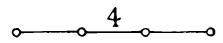
\includegraphics[keepaspectratio]{images/part002_520d8dd1.jpg}}

\begin{enumerate}
\def\labelenumi{(\roman{enumi})}
\setcounter{enumi}{1}
\tightlist
\item
  若边 \(\{1,2\}\) 的阶为 5，则图是下列图之一：
\end{enumerate}

\pandocbounded{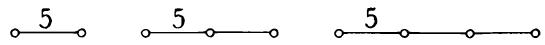
\includegraphics[keepaspectratio]{images/part002_9200390b.jpg}}

由引理 4，可设 \(l > 2\)。假设 \(\{i, i + 1\}\) 的阶为 \(\geqslant 4\)，其中 \(1 \leqslant i \leqslant l - 1\)。置

\(x = e_{1} + 2e_{2} + \dots + ie_{i}, y = e_{l} + 2e_{l - 1} + \dots + (l - i)e_{i + 1},\) 且 \(j = l - i\) .

根据引理 8，\(\| x\|^2 = \frac{1}{2} i(i + 1),\| y\|^2 = \frac{1}{2} j(j + 1)\)。另一方面，\((x|y) = ij(e_i|e_{i + 1}) = -ij\cos \frac{\pi}{m}\)，其中 \(m = 4\) 或 5（引理 4）。现在

\[
(x | y) ^ {2} <   \left\| x \right\| ^ {2} \| y \| ^ {2}.
\]

这给出

\[
\frac {1}{4} i j (i + 1) (j + 1) > i ^ {2} j ^ {2} \cos^ {2} \frac {\pi}{m}
\]

所以

\[
(i + 1) (j + 1) > 4 i j \cos^ {2} \frac {\pi}{m} \geqslant 2 i j.
\]

首先得到 \(ij - i - j - 1 < 0\)，或 \((i - 1)(j - 1) < 2\)。若

\[
1 <   i <   l - 1,
\]

则 \(1 < j < l - 1\)，所以 \(i = j = 2\)，从而 \({}^1\)

\[
9 > 16 \cos^ {2} {\frac {\pi}{m}}, \text {thus} \cos^ {2} {\frac {\pi}{m}} <   \cos^ {2} {\frac {\pi}{5}}
\]

从而 \(m = 4\)。这证明了 (i)。若 \(i = 1\) 且 \(m = 5\)，则 \(2j + 2 > 4j\frac{3 + \sqrt{5}}{8}\)，或 \(j\frac{\sqrt{5} - 1}{2} < 2\)，\(j < \sqrt{5} + 1 < 4\)，所以 \(l = j + 1 \leqslant 4\)。这证明了 (ii)。

引理 10. 若 X 有一个分叉点 i，则完全子图 \(X - \{i\}\) 是三条链的并；若 p - 1、q - 1、r - 1 是这些链的长度，则三元组 \(\{p, q, r\}\) 在置换意义下等于下列三元组之一：\(\{1, 2, 2\}\)、\(\{1, 2, 3\}\)、\(\{1, 2, 4\}\)、\(\{1, 1, m\}\)（某个 \(m \geqslant 1\)）。

顶点 \(i\) 属于 3 条边（引理 2），且没有其他分叉点（引理 7），所以完全子图 \(\mathrm{X} - \{i\}\) 是 3 条链 \(\mathrm{X}_1\)、\(\mathrm{X}_2\)、\(\mathrm{X}_3\) 的并，其中每条链都有一个与 \(i\) 在 \(\mathrm{X}\) 中相连的端点。设 \(\{i_1, i_2\}\)、\(\{i_2, i_3\}, \ldots, \{i_{p-1}, i_p\}\) 是 \(\mathrm{X}_1\) 的边，\(\{j_1, j_2\}\)、\(\{j_2, j_3\}, \ldots, \{j_{q-1}, j_q\}\) 是 \(\mathrm{X}_2\) 的边，\(\{k_1, k_2\}\)、\(\{k_2, k_3\}, \ldots, \{k_{r-1}, k_r\}\) 是 \(\mathrm{X}_3\) 的边，其中 \(i_1, j_1, k_1\) 与 \(i\) 在 \(\mathrm{X}\) 中相连。可设 \(p \geqslant q \geqslant r \geqslant 1\)。置

\[
\begin{array}{l} x = e _ {i _ {p}} + 2 e _ {i _ {p - 1}} + \dots + p e _ {i _ {1}} \\ y = e _ {j _ {q}} + 2 e _ {j _ {q - 1}} + \dots + q e _ {j _ {1}} \\ z = e _ {k _ {r}} + 2 e _ {k _ {r - 1}} + \dots + r e _ {k _ {1}}. \end{array}
\]

由于 X 的所有边的阶都是 3（引理 7），由引理 8 得 \(\| x\|^2 = \frac{1}{2} p(p + 1)\)、\(\| y\|^2 = \frac{1}{2} q(q + 1)\)、\(\| z\|^2 = \frac{1}{2} r(r + 1)\)。另一方面，\(e_i\) 与 \(e_{i_2}, e_{i_3}, \ldots, e_{i_p}\) 正交，故 \((e_i|x) = p(e_i|e_{i_1}) = -\frac{1}{2} p\)；同理 \((e_i|y) = -\frac{1}{2} q\)、\((e_i|z) = -\frac{1}{2} r\)。单位向量 \(\| x\|^ {-1}x\)、\(\| y\|^ {-1}y\)、\(\| z\|^ {-1}z\) 两两正交，且 \(e_i\) 不属于它们生成的子空间 F；从 \(e_i\) 到 F 的距离的平方为

\[
\begin{array}{r l} 1 - (e _ {i} | \frac {x}{\| x \|}) ^ {2} - (e _ {i} | \frac {y}{\| y \|}) ^ {2} - (e _ {i} | \frac {z}{\| z \|}) ^ {2} \\ & = 1 - \frac {1}{2} \frac {p}{p + 1} - \frac {1}{2} \frac {q}{q + 1} - \frac {1}{2} \frac {r}{r + 1} \\ & = 1 - \frac {1}{2} + \frac {1}{2} \frac {1}{p + 1} - \frac {1}{2} + \frac {1}{2} \frac {1}{q + 1} - \frac {1}{2} + \frac {1}{2} \frac {1}{r + 1}. \end{array}
\]

由于此量为 \(>0\)，有

\[
(p + 1) ^ {- 1} + (q + 1) ^ {- 1} + (r + 1) ^ {- 1} > 1.\tag{4}
\]

因此 \(3(r + 1)^{-1} > 1\)，所以 \(r < 2\)，最后 \(r = 1\)。于是由 (4) 得

\[
(p + 1) ^ {- 1} + (q + 1) ^ {- 1} > \frac {1}{2}\tag{5}
\]

故 \(2(q + 1)^{-1} > \frac{1}{2}\)，所以 \(q \leqslant 2\)。最后，若 \(q = 2\)，由 (5) 得

\[
(p + 1) ^ {- 1} > \frac {1}{6}. \quad \text { hence } p \leqslant 4.
\]

定理 1. 任一不可约有限 Coxeter 系统 (W.S) 的图同构于下列图之一：

\pandocbounded{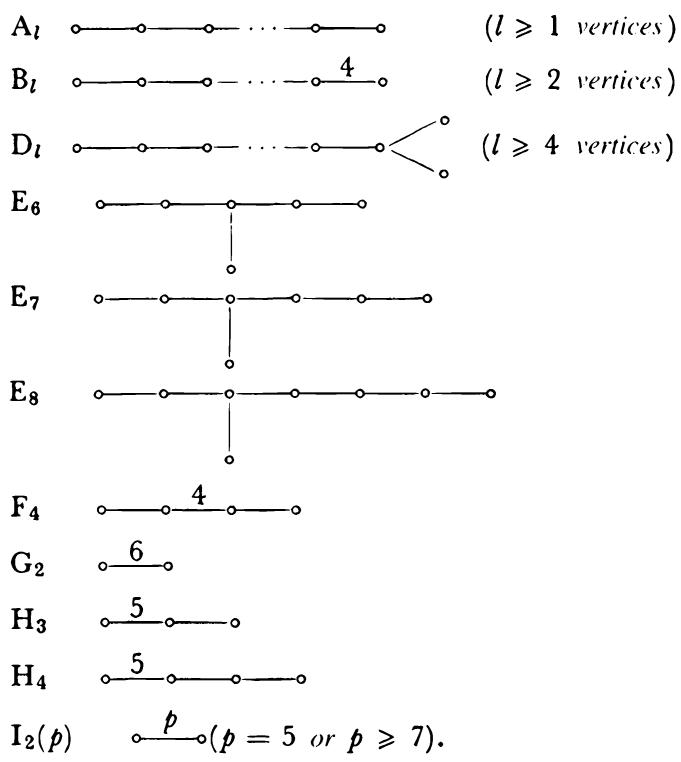
\includegraphics[keepaspectratio]{images/part002_677d99d4.jpg}}

这些图中任意两个都不同构。

事实上，设 \(\mathrm{W} = (m_{ij})\) 是 (W,S) 的 Coxeter 矩阵，且 \(l = \operatorname{Card}(S)\)。若某个 \(m_{ij}\) 为 \(\geqslant 6\)，则 l = 2（引理 4），且 (W,S) 的 Coxeter 图是 \(G_{2}\) 型或 \(I_{2}(p)\) 型，其中 \(p \geqslant 7\)。现在假设所有 \(m_{ij} \leqslant 5\)。

\begin{enumerate}
\def\labelenumi{\alph{enumi})}
\item
  若 \(m_{ij}\) 不全都等于 3，则 (W.S) 的图 X 是一条链，且恰有一个 \(m_{ij}\) 等于 4 或 5（引理 7）。若某个 \(m_{ij}\) 等于 5，则引理 9 表明我们得到 \(H_{3}\)、\(H_{4}\) 或 \(I_{2}(5)\) 型之一。若某个 \(m_{ij}\) 等于 4，则引理 9 表明我们得到 \(B_{l}\) 或 \(F_{4}\) 型之一。
\item
  现在假设所有 \(m_{ij}\) 都等于 3。若 X 是一条链，则 Coxeter 图是 \(A_{l}\) 型。否则，引理 10 表明它是 \(E_{6}\)、\(E_{7}\)、\(E_{8}\) 或 \(D_{l}\) 型。
\end{enumerate}

显然，所列 Coxeter 图中任意两个都不同构。

反之：

定理 2. 定理 1 中由 Coxeter 图 \(\mathbf{A}_l, \mathbf{B}_l, \ldots, \mathbf{I}_2(p)\) 定义的 Coxeter 群是有限的。

对于 \(I_{2}(p)\) 这显然成立，因为相应的群是阶为 2p 的二面体群（第四章第 1 节第 9 号）。对于 \(H_{4}\)，相应的二次型

为

\[
\begin{array}{r l} & \xi_ {1} ^ {2} + \xi_ {2} ^ {2} + \xi_ {3} ^ {2} + \xi_ {4} ^ {2} - \xi_ {1} \xi_ {2} - \xi_ {2} \xi_ {3} - 2 (\cos \frac {\pi}{5}) \xi_ {3} \xi_ {4} \\ & = \xi_ {1} ^ {2} + \xi_ {2} ^ {2} + \xi_ {3} ^ {2} + \xi_ {4} ^ {2} - \xi_ {1} \xi_ {2} - \xi_ {2} \xi_ {3} - \frac {1 + \sqrt {5}}{2} \xi_ {3} \xi_ {4} \\ & = (\xi_ {2} - \frac {\xi_ {1} + \xi_ {3}}{2}) ^ {2} + (\xi_ {4} - \frac {1 + \sqrt {5}}{4} \xi_ {3}) ^ {2} + \frac {3}{4} (\xi_ {1} - \frac {1}{3} \xi_ {3}) ^ {2} + \frac {7 - 3 \sqrt {5}}{24} \xi_ {3} ^ {2}. \end{array}
\]

由于 \(7 - 3\sqrt{5}\) 为 \textgreater0，此形式正且非退化，故相应的 Coxeter 群是有限的。\(H_{3}\) 所对应的情形也如此，因为它同构于前一个群的子群（第四章第 1 节第 8 号）。

对于 \(A_{l}\)、\(B_{l}, \ldots, G_{2}\) 型，我们将在第 5 至 13 号中构造以相应群为韦伊群的根系。我们将看到，这些群不仅有限，而且是晶体群（第 2 节，第 5 号）。

\subsection{Dynkin 图}

依照通常的语言滥用，我们称具有以下性质的一对 \((\Gamma, f)\) 为赋范图：

\begin{enumerate}
\def\labelenumi{\arabic{enumi})}
\item
  \(\Gamma\) 是一个图（称为 \((\Gamma, f)\) 的底图）。
\item
  若 E 表示有序对 \((i,j)\) 所成的集合，其中 \(\{i,j\}\) 是 \(\Gamma\) 的一条边，则 f 是从 E 到 R 的映射，并且有 \(f(i,j)f(j,i)=1\)（对所有 \((i,j)\in\mathbf{E}\)）。
\end{enumerate}

赋范图的同构概念是显然的。

设 R 是实向量空间 V 中的一个约化根系。我们将与之关联一个赋范图 \((X, f)\)，称为 R 的 Dynkin 图。X 的顶点将是 W(R) 在 \(\{B\} \times B\) 的并集（其中 B 为 R 的基集）中的轨道集 I 的元素。若 \(N = (n_{ij})_{i,j \in I}\)（分别为 \(M = (m_{ij})_{i,j \in I}\)）是 R 的典范 Cartan 矩阵（分别为 Coxeter 矩阵）（\(\S\) 1，第 5 号，备注 7），则 X 的两个顶点 i 和 j 相连，当且仅当 \(n_{ij} \neq 0\)，并置

\[
f (i, j) = \frac {n _ {i j}}{n _ {j i}}.
\]

由于 \(n_{ij} = 0\) 蕴含 \(n_{ji} = 0\)，这定义了一个赋范图 (X. f)。

设 \((x|y)\) 是 V 上在 W(R) 下不变的标量积，令 \(B = (\alpha_i)_{i \in I}\) 为 R 的一组按典范方式编号的基。第 1 节第 1 号的公式 (7) 和 (9) 表明，图 X 的顶点 i 和 j 相连，当且仅当

\[
(\alpha_ {i} | \alpha_ {j}) \neq 0
\]

并且

\[
f (i, j) = \frac {\left(\alpha_ {j} \mid \alpha_ {i}\right)}{\left(\alpha_ {j} \mid \alpha_ {j}\right)}.
\]

根据第 1 节第 3 号和第 5 号的结果，除交换 \(i\) 和 \(j\) 外，只有以下可能性：

\begin{enumerate}
\def\labelenumi{\arabic{enumi})}
\item
  \(i\) 和 \(j\) 不相连；\(n_{ij} = n_{ji} = 0\)；\(m_{ij} = 2\)；
\item
  \(f(i,j) = f(j,i) = 1; n_{ij} = n_{ji} = -1; m_{ij} = 3;\)
\item
  \(f(i,j) = 2\)，\(f(j,i) = 1/2\)；\(n_{ij} = -2\)。\(n_{ji} = -1\)；\(m_{ij} = 4\)；
\end{enumerate}

\[
f (i, j) = 3, f (j, i) = 1 / 3: n _ {i j} = - 3, n _ {j i} = - 1; m _ {i j} = 6.
\]

由此可见，Dynkin 图 R 确定 R 的 Cartan 矩阵和 Coxeter 矩阵，因而将 R 确定到同构为止。更精确地说，第 1 节第 5 号命题 15 的推论蕴含以下结果：

命题 1. 设 \(R_{1}\) 和 \(R_{2}\) 是向量空间 \(V_{1}\) 和 \(V_{2}\) 中的两个约化根系。设 \(B_{1} = (\alpha_{i})_{i \in I_{1}}\) 和 \(B_{2} = (\alpha_{i})_{i \in I_{2}}\) 分别为 \(R_{1}\) 和 \(R_{2}\) 的按典范方式编号的基。设 \(\lambda\) 是从 \(R_{1}\) 的 Dynkin 图到 \(R_{2}\) 的 Dynkin 图的同构。则存在唯一的从 \(V_{1}\) 到 \(V_{2}\) 的同构，将 \(R_{1}\) 变为 \(R_{2}\)，并且将 \(\alpha_{i}\) 变为 \(\alpha_{\lambda(i)}\)（对所有 \(i \in I_{1}\)）。

显然，R 的一个自同构定义 R 的 Dynkin 图的一个自同构，从而定义从群 A(R) 到 R 的 Dynkin 图自同构群的同态 \(\varphi\)。

推论。同态 \(\varphi\) 通过取商定义了从群 A(R)/W(R) 到 R 的 Dynkin 图自同构群的一个同构。

显然，\(\varphi(g) = \operatorname{Id}\)（对所有 \(g \in W(R)\)）。另一方面，命题 1 表明，存在一个同构 \(\psi\)，它从 \(R\) 的 Dynkin 图同构群映到 \(E\)，而 \(A(R)\) 中固定给定基 \(B\)（属于 \(R\)）的元素组成此子群，并且满足 \(\varphi \circ \psi = \operatorname{Id}\)。由于 \(A(R)\) 是 \(E\) 与 \(W(R)\) 的半直积（第 1 节，第 5 号，命题 16），推论得证。

实际上，Dynkin 图 \((X, f)\) 用由节点和边组成的图表示如下。节点对应于 X 的顶点；在上述情形 1）、2）、3）和 4）中，分别用 0、1、2 或 3 条边连接对应于两个不同顶点 i 和 j 的两个节点（除交换 i 和 j 外）。此外，在情形 3）和 4）中，即当 \(f(i, j) > 1\)，或根 \(\alpha_{1}\) 与 \(\alpha_{j}\) 不正交且长度不同时，在连接对应于 i 和 j 的节点的双边或三边上放置不等号 \textgreater{}，方向指向对应于 j 的节点（即较短的根）：

\[
\underset {i} {\longrightarrow} \underset {j} {\longrightarrow} \quad (\text { for   } f (i, j) = 2), \quad \underset {i} {\longrightarrow} \underset {j} {\longrightarrow} \quad (\text { for   } f (i, j) = 3).
\]

显然，可以从此图恢复 Dynkin 图 \((X, f)\)。

注意，与 W(R) 的 Coxeter 图对应的图可以从与 R 的 Dynkin 图对应的图得到：保留节点和单边，并将双边（分别为三边）替换为上方标有数字 4（分别为 6）的边。反过来，给定 W(R) 的 Coxeter 图，可以使用此过程的逆过程恢复与 R 的 Dynkin 图对应的图，但双边或三边上的不等号除外。因此定理 1 立即给出可能的 Dynkin 图列表。更精确地说：

定理 3. 若 R 是不可约约化根系，则其 Dynkin 图同构于以下图示中的某一个图：

\pandocbounded{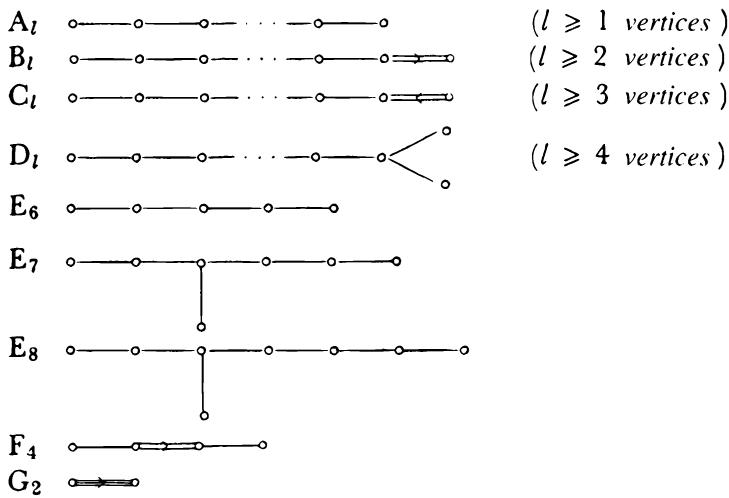
\includegraphics[keepaspectratio]{images/part002_c37a5a77.jpg}}

这些图中任意两个都不同构，并且存在不可约约化根系，使每一个图（在同构意义下）都成为其 Dynkin 图。

第一个断言立即由定理 1、上述备注、图 \(H_{3}\)、\(H_{4}\) 和 \(I_{2}(p)\) 的 Coxeter 群（当 p = 5 及 \(p \geqslant 7\) 时）不是晶体群这一事实，以及与 Coxeter 图 \(F_{4}\)（分别为 \(G_{2}\)）对应的 Dynkin 图的双边（分别为三边）的两种可能不等号给出同构 Dynkin 图这一事实得到。第二个断言是显然的，第三个断言将由对每一种类型明确构造一个不可约约化根系而得出；这一构造将在第 5 至 13 号中进行。

备注。1）图 \(A_{1}\) 退化为一个节点；也记为 \(B_{1}\) 或 \(C_{1}\)。图 \(B_{2}\) 也记为 \(C_{2}\)。图 \(A_{3}\) 也记为 \(D_{3}\)。最后，\(D_{2}\) 表示由两个不相连节点组成的图。（这些约定源于相应根系的性质，参见第 5 至 8 号。）

\begin{enumerate}
\def\labelenumi{\arabic{enumi})}
\setcounter{enumi}{1}
\tightlist
\item
  若 \((X, f)\) 是约化根系 R 的 Dynkin 图，则对偶根系的 Dynkin 图可与 \((X, f^{-1})\) 认同。换言之，与 \(R^{\prime}\) 的 Dynkin 图对应的图可以从与 R 的 Dynkin 图对应的图得到，只需反转不等号。若 R 不可约，则可见 R 与 \(R^{\prime}\) 同构，除非 R 是 \(B_{l}\) 型或 \(C_{l}\) 型；在这两种情形下，\(R^{\prime}\) 分别是 \(C_{l}\) 型或 \(B_{l}\) 型。
\end{enumerate}

\subsection{仿射韦伊群与完备 Dynkin 图}

设 R 是不可约约化根系，\((\mathbf{X}, f)\) 是其 Dynkin 图。我们将定义另一个赋范图 \((\tilde{\mathbf{X}}, \tilde{f})\)，称为 R 的完备 Dynkin 图。\(\tilde{I}\) 是 \(\tilde{X}\) 的顶点集，由 X 的顶点集 I 和一个记为 0 且不属于 I 的顶点组成。为定义 \(\tilde{f}\)，选取 R 的一组基 \(B = (\alpha_{i})_{i \in I}\) 以及在 W(R) 下不变的标量积 \((x|y)\)。令 \(\alpha_{0}\) 为相对于 B 所定义的序的最高根的负根。两个不同顶点 \(i, j \in \tilde{I}\) 相连，当且仅当 \((\alpha_{i}|\alpha_{j}) \neq 0\)，并置

\[
\tilde {f} (i, j) = \frac {\left(\alpha_ {i} \mid \alpha_ {i}\right)}{\left(\alpha_ {j} \mid \alpha_ {j}\right)}.
\]

立即可见，这样定义的图 \(\tilde{X}\) 和映射 \(\tilde{f}\) 不依赖于 B 或标量积的选择。

若秩 \(l\) 的 \(R\) 等于 1，则 \(I = \{i\}\) 且 \(\alpha_0 = -\alpha_1\)；故 \(\tilde{f}(0, i) = 1\)。若 \(l \geqslant 2\)，\(\alpha_0\) 不与任何 \(\alpha_i\) 成比例，且 \((\alpha_0|\alpha_i)\) \(\leqslant 0\)（第 1 节，第 8 号，命题 25）。对于任意一对不同元素 \((i,j)\)（属于 \(\tilde{I}\)），唯一可能性就是前一号中标为 1）、2）、3）、4）的那些可能性（例如置 \(n_{0i} = n(\alpha_0, \alpha_i)\)，\(m_{0i} = \text{阶 } s_{\alpha_0}s_{\alpha_i}\)，其中 \(i \in I\)）。

在 \(l \geqslant 2\) 的情形，完备 Dynkin 图用与前一号相同约定的图表示，有时用虚线表示连接顶点 0 与其他顶点的边。注意，若这种边上存在不等号 \textgreater{}，它总是指向异于 0 的顶点，因为 \(\alpha_{0}\) 是最长根（\(\S\) 1，第 8 号，命题 25）。图 \((\mathbf{X}, f)\) 是从 \((\tilde{\mathbf{X}}, f)\) 删除顶点 0 后得到的子图。

A(R) 在 (X. f) 上的作用延拓为 \((\tilde{\mathbf{X}}.\tilde{f})\) 上的作用，并固定 0；而 W(R) 在 \((\tilde{\mathbf{X}}.\tilde{f})\) 上平凡作用。

我们沿用第 2 节的记号。第 2 节第 2 号的命题 5，连同第五章第 3 节第 2 号的定理 1，表明，仿射韦伊群的 Coxeter 图 \(\Sigma\) 与 \(W_{a}(R)\) 相关；它可以从 \((\tilde{X},\tilde{f})\) 按照由 \(W(R)\) 从 \((X,f)\) 得到其 Coxeter 图的相同规则得到。另一方面，令 G 为 \(W_{a}(R)\) 的正规化子（第 2 节，第 3 号）。对每个 \(g\in G\)，都有一个自同构 \(\varphi(g)\) 作用于 \(\Sigma\)，且 \(\varphi(g)=\mathrm{Id}\)（若 \(g\in W_{a}(R)\)）。反过来，给定 \(\lambda\)，它是 \(\Sigma\) 的一个自同构；根据第五章第 4 节第 9 号的命题 11，存在唯一元素 \(g=\psi(\lambda)\)，保持给定小室 C，并满足 \(\varphi(g)=\lambda\)。由于 G 是保持 C 的元素所成的子群 \(G_{C}\) 与 \(W_{a}(R)\) 的半直积（第 2 节，第 3 号），故 \(\varphi\) 通过取商定义了从 \(G/W_{a}\)（或从 \(G_{C}\)）到 \(\operatorname{Aut}(\Sigma)\) 的同构。立即可见，这个同构与从 A(R)/W(R) 到 G/ \(W_{a}\) 的典范映射的复合，恰好是从 A(R)/W(R) 到 \(\operatorname{Aut}(\Sigma)\) 的同态；这个同态由上面定义的从 A(R)/W(R) 到 \(\operatorname{Aut}(\tilde{X},\tilde{f})\) 的同态所诱导。根据第 2 节第 3 号，群 \(\operatorname{Aut}(\Sigma)\) 同构于

\(A(R)/W(R)\) 与 \(P(R')/Q(R')\) 的半直积，而 \(P(R')/Q(R')\) 同构于群 \(I_{C'} = G_{C'} \cap W_{a}'\)（记号同第 2 节第 3 号）：\(\text{Aut}(\Sigma)\) 中与 \(\gamma_{i}\)（\(I_{C}\) 中的元素）相对应的元素，将顶点 0 变为 \(\Sigma\) 的顶点 i。

备注。可以证明，典范映射

\[
\operatorname{Aut} (\tilde {X}, \tilde {f}) \rightarrow \operatorname{Aut} (\Sigma)
\]

是一个同构。

定理 4. 设 (W.S) 是 S 有限的不可约 Coxeter 系统。关联的二次型（第五章第 4 节第 1 号）正且退化，当且仅当 (W.S) 的 Coxeter 图同构于下列图之一：

\pandocbounded{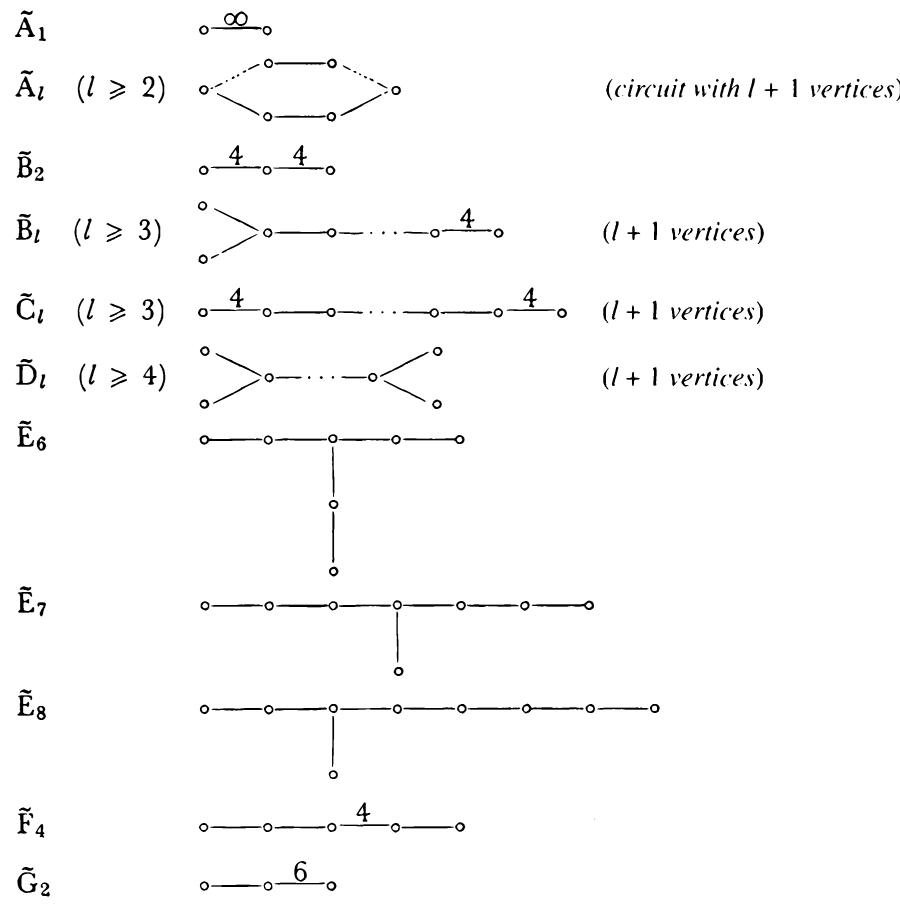
\includegraphics[keepaspectratio]{images/part002_b5f8d83f.jpg}}

这些 Coxeter 图中任意两个都不同构。

根据第五章第 4 节第 9 号以及第 2 节第 5 号的命题 8，二次型正且退化的 Coxeter 系统正是对应于不可约约化根系的仿射韦伊群的那些系统。因此，定理由下面第 5 至 13 号中对完备 Dynkin 图的确定得出。

\subsection{根系构造的预备知识}

设 V 是一个维数 \(l \geqslant 1\) 的实向量空间，并配备标量积 \((x|y)\)。设 L 是 V 的离散子群，A 是一个有限的数集，且其中每个数为 \textgreater0；R 是由这样的元素组成的集合：\(\alpha \in L\)，且 \((\alpha|\alpha) \in \Lambda\)。假设 R 生成 V，并且对于 R 中任意一对点 \((\alpha,\beta)\)，数 \(2\frac{(\alpha|\beta)}{(\alpha|\alpha)}\) 是整数。则 R 是 V 中的根系。事实上，R 显然满足 \((RS_{I})\)。令 \(\alpha \in R\)：令 \(s_{\alpha}\) 为正交反射 \(x \mapsto x - 2\frac{(x|\alpha)}{(\alpha|\alpha)}\alpha\)；于是若 \(\beta \in R\)，有 \(2\frac{(\beta|\alpha)}{(\alpha|\alpha)} \in Z\)，故 \(s_{\alpha}(\beta) \in L\)，且 \(\|s_{\alpha}(\beta)\| = \| \beta \|\)，所以 \(s_{\alpha}(\beta) \in R\)；因此 R 满足 \((RS_{II})\) 和 \((RS_{III})\)，并且若 A 不含形如 \(\lambda\) 和 \(4\lambda\) 的两个数，则 R 是约化的。

现在令 V 为 \(E = R^{n}\) 的一个子空间。令 \((\varepsilon_{1}, \ldots, \varepsilon_{n})\) 为 E 的典范基；在 E 上取使此基成为标准正交基的标量积，并借助此标量积将 \(E^{*}\) 与 E（分别将 \(V^{*}\) 与 V）认同。定义 E 的子群 \(L_{0}, L_{1}, L_{2}, L_{3}\) 如下：

\begin{enumerate}
\def\labelenumi{\arabic{enumi})}
\item
  \(L_{0}\) 是以 \((\varepsilon_{i})\) 为基的 Z-模。我们有 \((\alpha|\beta)\in\mathbf{Z}\)，其中 \(\alpha,\beta\in L_{0}\)。满足条件 \(\alpha\in L_{0}\) 且 \((\alpha|\alpha)=1\) 的向量是 \(\pm\varepsilon_{i}\;(1\leqslant i\leqslant n)\)；满足 \((\alpha|\alpha)=2\) 的向量是 \(\pm\varepsilon_{i}\pm\varepsilon_{j}\)，其中 i\textless j（\(\pm\) 中的两个符号，在 \(\pm\varepsilon_{i}\pm\varepsilon_{j}\) 中彼此独立选取；本节其余部分均采用类似约定）。
\item
  \(L_{1}\) 是 \(L_{0}\) 的 Z-子模，由 \(x = \sum_{i=1}^{n} \xi_{i} \varepsilon_{i} \in L_{0}\) 组成，其中 \(\sum_{i=1}^{n} \xi_{i}\) 为偶数；由于 \(\xi_{i}\) 与 \(\xi_{i}^{2}\) 具有相同的奇偶性，这等价于要求 \((x|x)\) 为偶数。令 \(L_{1}^{\prime}\) 为 \(L_{1}\) 的子模，由 \(\varepsilon_{i} \pm \varepsilon_{j}\) 生成；我们有 \(\sum_{i=1}^{n} \xi_{i} \varepsilon_{i} \equiv (\sum_{i=1}^{n} \xi_{i}) \varepsilon_{n} \pmod{L_{1}^{\prime}}\)，且由于 \(2\varepsilon_{n} = (\varepsilon_{1} + \varepsilon_{n}) - (\varepsilon_{1} - \varepsilon_{n}) \in L_{1}^{\prime}\)，可知 \(L_{1}^{\prime} = L_{1}\)。由于 \(L_{0}\) 由 \(L_{1}\) 和 \(\varepsilon_{1}, L_{0}/L_{1}\) 生成，后者同构于 Z/2Z。
\item
  \(\mathrm{L}_2 = \mathrm{L}_0 + \mathbf{Z}\left(\frac{1}{2} \sum_{i=1}^{n} \varepsilon_i\right)\)。显然，元素 \(x = \sum_{i=1}^{n} \xi_i \varepsilon_i\) 属于 \(\mathrm{V}\)，它属于 \(\mathrm{L}_2\) 当且仅当
\end{enumerate}

\[
2 \xi_ {i} \in \mathbf {Z}, \quad \xi_ {i} - \xi_ {j} \in \mathbf {Z} \text {   for   all   } i \text {   and   } j.\tag{6}
\]

由于 \((\varepsilon_k|_{\frac{1}{2}}\sum_{i=1}^{n}\varepsilon_i) = \frac{1}{2}\) 对所有 \(k\) 成立，且 \(\| \frac{1}{2}\sum_{i=1}^{n}\varepsilon_i\|^2 = \frac{n}{4}\)，有 \((\alpha|\beta) \in \frac{1}{2}\mathbf{Z}\) 对于 \(\alpha, \beta \in L_2\) 成立，其中 \(n\) 为偶数。群 \(L_2 / L_0\) 同构于 \(\mathbf{Z}/2\mathbf{Z}\)。

\begin{enumerate}
\def\labelenumi{\arabic{enumi})}
\setcounter{enumi}{3}
\tightlist
\item
  \(L_{3} = L_{1} + \mathbf{Z}\left(\frac{1}{2} \sum_{i=1}^{n} \varepsilon_{i}\right)\)。若 n 是 4 的倍数，则 \(L_{3}\) 是由 \(\sum_{i=1}^{n} \xi_{i} \varepsilon_{i}\) 组成的集合，这些元素满足 (6) 以及条件 \(\sum_{i=1}^{n} \xi_{i} \in 2\mathbf{Z}\)；在此情形，\((\alpha | \beta) \in \mathbf{Z}\) 对所有 \(\alpha, \beta \in L_{3}\) 成立。
\end{enumerate}

立即可见，与 \(L_{0}\)（分别为 \(L_{1}, L_{2}\)）关联的 E 的子群是 \(L_{0}\)（分别为 \(L_{2}, L_{1}\)）。与 \(L_{3}\) 关联的 E 的子群是

\[
x = \sum_ {i = 1} ^ {n} \xi_ {i} \varepsilon_ {i} \in L _ {2}
\]

满足 \((x|\frac{1}{2}\sum_{i = 1}^{n}\varepsilon_i)\in \mathbf{Z}\)，即满足 \(\sum_{i = 1}^{n}\xi_{i}\in 2\mathbf{Z}\)；因此若 \(n\equiv 0\)（模 4），这个关联子群就是 \(\mathrm{L}_3\)。

阿贝尔群 \(\mathrm{L}_2 / \mathrm{L}_1\) 的阶为 4，因而同构于 \(\mathbf{Z} / 4\mathbf{Z}\) 或 \(\mathbf{Z} / 2\mathbf{Z} \times \mathbf{Z} / 2\mathbf{Z}\)（《代数》第七章第 4 节第 6 号定理 3）。若 \(n\) 为奇数，

\[
p (\frac {1}{2} \sum_ {i = 1} ^ {n} \varepsilon_ {i}) \in \mathrm{L} _ {1} \Leftrightarrow p \equiv 0 (\mathrm{mod.} 4)
\]

所以 \(\mathrm{L}_2 / \mathrm{L}_1\) 是 4 阶循环群。若 \(n\) 为偶数，

\[
p (\frac {1}{2} \sum_ {i = 1} ^ {n} \varepsilon_ {i}) \in \mathrm{L} _ {1} \Leftrightarrow p \equiv 0 (\mathrm{mod.} 2)
\]

所以 \(L_{2}/L_{1}\) 含有两个不同的 2 阶元素，并同构于 \(Z/2Z \times Z/2Z\)。

在下面九个号以及各图版中，我们将一直使用这些记号。对于定理 3 中的每一种 Dynkin 图，我们将明确描述：

\begin{enumerate}
\def\labelenumi{(\Roman{enumi})}
\item
  一个根系 R 及其根的数目。
\item
  R 的一组基 B 及相应的正根。基 B 将用整数 \(1,\ldots,l\) 编号。
\item
  Coxeter 数 \(h\)（第 1 节，第 11 号）。
\item
  最高根 \(\tilde{\alpha}\)（相对于 B 所定义的序）及完备 Dynkin 图（第 3 号）。我们将在每个顶点旁标出 B 中对应的根。
\item
  对偶根系 \(\mathbb{R}^{\prime}\)、典范双线性形式以及常数 \(\gamma(\mathbb{R})\)（第 1 节，第 12 号）。
\item
  相对于 B 的基本权（第 1 节，第 10 号）。
\item
  正根之和。
\item
  群 \(P(R), Q(R), P(R)/Q(R)\) 以及连接指标（第 1 节，第 9 号）。
\item
  \(\mathrm{W}(\mathrm{R})\) 的指数（第五章第 6 节第 2 号定义 2）。在 \(\mathbf{A}_l, \mathbf{B}_l, \mathbf{C}_l\) 和 \(\mathbf{D}_l\) 的情形，我们确定其对称不变量。
\item
  W(R) 的阶（以及在某些情形下它的结构）。
\item
  群 \(A(R)/W(R)\)、它在 Dynkin 图上的作用，以及将 B 变为 -B 的元素 \(w_{0}\)（属于 \(W(R)\)）。
\item
  \(\mathrm{P}(\mathrm{R}^{\prime})/\mathrm{Q}(\mathrm{R}^{\prime})\) 在完备 Dynkin 图上的作用，以及 \(\mathrm{A}(\mathrm{R})/\mathrm{W}(\mathrm{R})\) 在 \(\mathrm{P}(\mathrm{R}^{\prime})/\mathrm{Q}(\mathrm{R}^{\prime})\) 上的作用。
\end{enumerate}

对于定理 3 中的每个 Dynkin 图，这些数据将汇集于图版 I 至 IX 中，并按上述统一方式排列。我们还给出：

\begin{enumerate}
\def\labelenumi{(\Roman{enumi})}
\setcounter{enumi}{12}
\tightlist
\item
  Cartan 矩阵，由它按第 2 号所述方式导出 Dynkin 图。
\end{enumerate}

\subsection{\texorpdfstring{\(B_{l}\) 型根系（\(l \geqslant 2\)）}{B\_l 型根系 (l >= 2)}}

\begin{enumerate}
\def\labelenumi{(\Roman{enumi})}
\item
  我们考虑 \(L_{0}\)，它是 V = \(R^{l}\)（第 4 号）中的群。令 R 为由满足 \(\alpha \in L_{0}\) 且 \((\alpha|\alpha) = 1\) 或 \((\alpha|\alpha) = 2\) 的元素所成的集合，换言之，是由向量 \(\pm\varepsilon_{i}\)（\(1 \leqslant i \leqslant l\)）和 \(\pm\varepsilon_{i} \pm \varepsilon_{j}\)（\(1 \leqslant i < j \leqslant l\)）组成的集合。显然，R 生成 V，且 \(2(\alpha|\beta)/(\alpha|\alpha) \in \mathbf{Z}\) 对所有 \(\alpha, \beta \in R\) 成立。因此 R 是 V 中的约化根系（第 4 号）。根的数目为 \(n = 2l + 4\frac{l(l-1)}{2} = 2l^{2}\)。
\item
  置
\end{enumerate}

\[
\alpha_ {1} = \varepsilon_ {1} - \varepsilon_ {2}, \alpha_ {2} = \varepsilon_ {2} - \varepsilon_ {3}, \dots , \alpha_ {l - 1} = \varepsilon_ {l - 1} - \varepsilon_ {l}, \alpha_ {l} = \varepsilon_ {l}.
\]

于是

\[
\begin{array}{c} \varepsilon_ {i} = \alpha_ {i} + \alpha_ {i + 1} + \dots + \alpha_ {l} \quad (1 \leqslant i \leqslant l) \\ \varepsilon_ {i} + \varepsilon_ {j} = (\alpha_ {i} + \alpha_ {i + 1} + \dots + \alpha_ {l}) + (\alpha_ {j} + \alpha_ {j + 1} + \dots + \alpha_ {l}) (1 \leqslant i <   j \leqslant l) \\ \varepsilon_ {i} - \varepsilon_ {j} = \alpha_ {i} + \alpha_ {i + 1} + \dots + \alpha_ {j - 1} \quad (1 \leqslant i <   j \leqslant l). \end{array}
\]

因此 \((\alpha_{1},\alpha_{2},\ldots ,\alpha_{l})\) 是 R 的一组基（第 1 节，第 7 号，命题 20 的推论 3）。此外，\(\| \alpha_{i}\|^{2} = 2\) 对 \(i < l\) 成立，\(\| \alpha_l\| ^2 = 1\)，\((\alpha_i|\alpha_{i + 1}) = -1\) 对 \(1\leqslant i\leqslant l - 1\) 成立，\((\alpha_i|\alpha_j) = 0\) 对 \(j > i + 1\) 成立：因此 R 的 Dynkin 图为 \(\mathbf{B}_l\) 型，这表明 R 不可约。正根是 \(\varepsilon_{i}\) 以及 \(\varepsilon_{i}\pm \varepsilon_{j}\)（\(i < j\)）。

\begin{enumerate}
\def\labelenumi{(\Roman{enumi})}
\setcounter{enumi}{2}
\tightlist
\item
  根据第五章第 6 节第 2 号定理 1 (ii)。
\end{enumerate}

\[
h = n / l = 2 l.
\]

\begin{enumerate}
\def\labelenumi{(\Roman{enumi})}
\setcounter{enumi}{3}
\tightlist
\item
  令 \(\tilde{\alpha} = \varepsilon_{1} + \varepsilon_{2} = \alpha_{1} + 2\alpha_{2} + 2\alpha_{3} + \cdots + 2\alpha_{l}\)，这是一个根。它相对于基 \((\alpha_{i})\) 的坐标之和为 2l - 1 = h - 1。根据第 1 节第 11 号命题 31，\(\tilde{\alpha}\) 是 R 的最高根。有 \((\tilde{\alpha}| \alpha_{i}) = 0\) 对 \(i \neq 2\) 成立，且 \((\tilde{\alpha}| \alpha_{2}) = 1\)。由于 \(\alpha_{2}\) 的长度分别为 1 和 \(\sqrt{2}\)，对应于 l = 2 和 \(l \geqslant 3\)，R 的完备 Dynkin 图如下：
\end{enumerate}

\[
\text { for } l = 2 \quad \alpha_ {2} \alpha_ {1}
\]

\pandocbounded{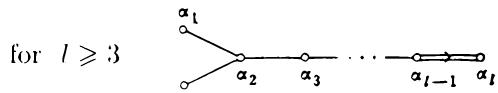
\includegraphics[keepaspectratio]{images/part002_79c781e2.jpg}}

\begin{enumerate}
\def\labelenumi{(\Alph{enumi})}
\setcounter{enumi}{21}
\tightlist
\item
  公式 \(\alpha^{\prime} = \frac{2\alpha}{(\alpha|\alpha)}\) 给出 \(R^{\prime}\) 的向量集：\(\pm 2\varepsilon_{i}\)（\(1 \leqslant i \leqslant l\)）以及 \(\pm \varepsilon_{i} \pm \varepsilon_{j}\)（\(1 \leqslant i < j \leqslant l\)）。\(R^{\prime}\) 的 Dynkin 图按照第 2 号所述过程由 \(R\) 的 Dynkin 图得到，并可见 \(R^{\prime}\) 为 \(C_{l}\) 型。
\end{enumerate}

有 \(4l - 2\) 个根不与 \(\beta = \varepsilon_1\) 正交，即 \(\pm \varepsilon_1\) 以及 \(\pm \varepsilon_1 \pm \varepsilon_j\)（\(2 \leqslant j \leqslant l\)）；对于每个这样的根 \(\alpha\)，\(n(\alpha, \beta) = \pm 2\)。第 1 节第 12 号的公式 (17) 表明，对于 \(\Phi_{\mathrm{R}}\)，\(\beta\) 的长度平方为 \((4l - 2)^{-1}\)；因此 \(\Phi_{\mathrm{R}}(x, y) = (x|y)/(4l - 2)\)。在 \(x = y = \beta\) 的情形应用第 1 节第 12 号的公式 (18)。这给出

\[
2 + \frac {1}{4} (4 l - 4) = \gamma (R) \frac {1}{4 l - 2}
\]

从而 \(\gamma(R) = (l + 1)(4l - 2)\)。

\begin{enumerate}
\def\labelenumi{(\Roman{enumi})}
\setcounter{enumi}{5}
\tightlist
\item
  基本权 \(\omega_{i}\)（\(1 \leqslant i \leqslant l\)）满足 \((\omega_{i}|\alpha_{j}) = \delta_{ij}\)，容易计算，得到
\end{enumerate}

\[
\begin{array}{l} \omega_ {i} = \varepsilon_ {1} + \varepsilon_ {2} + \dots + \varepsilon_ {i} \\ \qquad = \alpha_ {1} + 2 \alpha_ {2} + \dots + (i - 1) \alpha_ {i - 1} + i (\alpha_ {1} + \alpha_ {i + 1} + \dots + \alpha_ {l}) (i <   l) \\ \omega_ {l} = \frac {1}{2} (\varepsilon_ {1} + \varepsilon_ {2} + \dots + \varepsilon_ {l}) = \frac {1}{2} (\alpha_ {1} + 2 \alpha_ {2} + \dots + l \alpha_ {l}). \end{array}
\]

\begin{enumerate}
\def\labelenumi{(\Roman{enumi})}
\setcounter{enumi}{6}
\tightlist
\item
  正根之和为
\end{enumerate}

\[
\begin{array}{l} 2 \rho = (2 l - 1) \varepsilon_ {1} + (2 l - 3) \varepsilon_ {2} + \dots + 3 \varepsilon_ {l - 1} + \varepsilon_ {l} \\ = (2 l - 1) \alpha_ {1} + 2 (2 l - 2) \alpha_ {2} + \dots + i (2 l - i) \alpha_ {i} + \dots + l ^ {2} \alpha_ {l}. \end{array}
\]

\begin{enumerate}
\def\labelenumi{(\Roman{enumi})}
\setcounter{enumi}{7}
\item
  有 \(Q(R) = L_{0}\)（第 4 号），且 \(P(R)\) 由 \(Q(R)\) 和 \(\omega_{l}\) 生成，故等于 \(L_{2}\)（第 4 号）。因此，\(P(R)/Q(R)\) 同构于 Z/2Z，连接指标等于 2。
\item
  以及 (X) 在 \(R^{l}\) 中，正交反射 \(s_{\varepsilon_{i}-\varepsilon_{j}}\)（\(i \neq j\)）交换 \(\varepsilon_{i}\) 和 \(\varepsilon_{j}\)，并在指标 k 异于 i 和 j 时保持 \(\varepsilon_{k}\) 不变。\(s_{\varepsilon_{i}-\varepsilon_{j}}\) 生成一个群 \(G_{1}\)，它同构于对称群 \(S_{l}\)。正交反射 \(s_{\varepsilon_{i}}\) 将 \(\varepsilon_{i}\) 变为 \(-\varepsilon_{i}\)，并在指标 k 异于 i 时保持 \(\varepsilon_{k}\) 不变。\(s_{\varepsilon_{i}}\) 生成一个群 \(G_{2}\)，它同构于 \((\mathbf{Z}/2\mathbf{Z})^{l}\)。韦伊群 W(R) 由 \(G_{1}\) 和 \(G_{2}\) 生成，且 \(G_{2}\) 是 W(R) 的正规子群，所以 W(R) 同构于 \(S_{l}\) 与 \((\mathbf{Z}/2\mathbf{Z})^{l}\) 的半直积。因此它的阶为 \(2^{l}\cdot l!\)。
\end{enumerate}

对称代数 \(\mathbf{S}(\mathbf{R}^{l})\) 可典范地与多项式函数代数 \(\mathrm{P}(\xi_{1},\ldots,\xi_{l})\) 认同，后者定义在 \(R^{l}\) 上。要使这样的多项式在 \(\mathrm{W}(\mathrm{R})\) 下不变，首先必须有

\[
P \left(\xi_ {1}. \xi_ {2}. \dots ., \xi_ {l}\right) = P \left(\pm \xi_ {1}. \pm \xi_ {2}. \dots ., \pm \xi_ {l}\right)
\]

对右端的符号作任意选择均成立，从而

\[
\mathrm{P} \left(\xi_ {1}, \dots , \xi_ {l}\right) = \mathrm{Q} \left(\xi_ {1} ^ {2}, \dots , \xi_ {l} ^ {2}\right)
\]

其中 Q 是多项式，并且 Q 还是对称多项式；这些条件也是充分的。因此（《代数》第五章附录 I），\(\mathbf{S}(\mathbf{R}^{l})^{\mathrm{W}(\mathbb{R})}\) 是由以下 l 个多项式函数生成的代数

\[
t _ {i} = \sum_ {\tau \in \mathfrak {S} _ {l}} \xi_ {\tau (1)} ^ {2} \xi_ {\tau (2)} ^ {2} \dots \xi_ {\tau (l)} ^ {2} \quad (1 \leqslant i \leqslant l).
\]

此外，\(\mathbf{R}\) 上的 \(\mathbf{S}(\mathbf{R}^l)^{\mathrm{W(R)}}\) 的分式域的超越次数为 \(l\)，所以 \(t_i\) 代数独立。由于 \(t_i\) 的次数为 \(2,4,\ldots ,2l\)，我们得到 \(\mathrm{W(R)}\) 的指数（第五章第 6 节第 3 号命题 3）为：

\[
1, 3, 5, \dots , 2 l - 1.
\]

\begin{enumerate}
\def\labelenumi{(\Roman{enumi})}
\setcounter{enumi}{10}
\item
  Dynkin 图的唯一自同构是恒等元。因此，\(A(R) = W(R)\) 且 \(-1 \in W(R)\)。由于 -1 将 B 变为 -B，我们得到 \(w_{0} = -1\)。
\item
  群 \(P(R^{\prime})/Q(R^{\prime})\) 是 \(P(R)/Q(R)\) 的对偶，因而同构于 Z/2Z。其非平凡元置换对应于 \(\alpha_{0}\) 和 \(\alpha_{1}\) 的顶点，并固定其他顶点。
\end{enumerate}
